%=============================
%        Introduction
%=============================
\section{\review{Introduction}}

KEK, or the High Energy Accelerator Research Organization (Kō Enerugī Kasokuki Kenkyū Kikō), is a
Japanese institution operating the country's largest particle physics laboratory, located in
Tsukuba. KEK provides particle accelerators and essential infrastructure for a wide range of
research fields, including high-energy physics, material science, structural biology, and radiation
science. One of its most notable facilities is SuperKEKB, the world's most advanced
electron-positron collider. SuperKEKB is designed to reach an instantaneous luminosity of up to $80
\times 10^{34} \, \text{cm}^{-2}\text{s}^{-1}$ and has recently completed its commissioning phase.
It accelerates a 7 GeV electron beam in the High-Energy Ring (HER) and a 4 GeV positron beam in the
Low-Energy Ring (LER), which collide at a single interaction point where the Belle II experiment is
conducted. SuperKEKB currently holds the world record for instantaneous luminosity at $4.71 \times
10^{34} \, \text{cm}^{-2}\text{s}^{-1}$~\cite{zhou_luminosity_2023}, surpassing the previous record
set by the LHC.  With a circumference of approximately 3 km, it is the largest lepton collider in
operation.  Similar to CERN, KEK is a large complex housing multiple accelerators and facilities, as
shown in the schematic in \cref{fig:kek:layout_superkekb}.

\begin{figure}[!htb]
    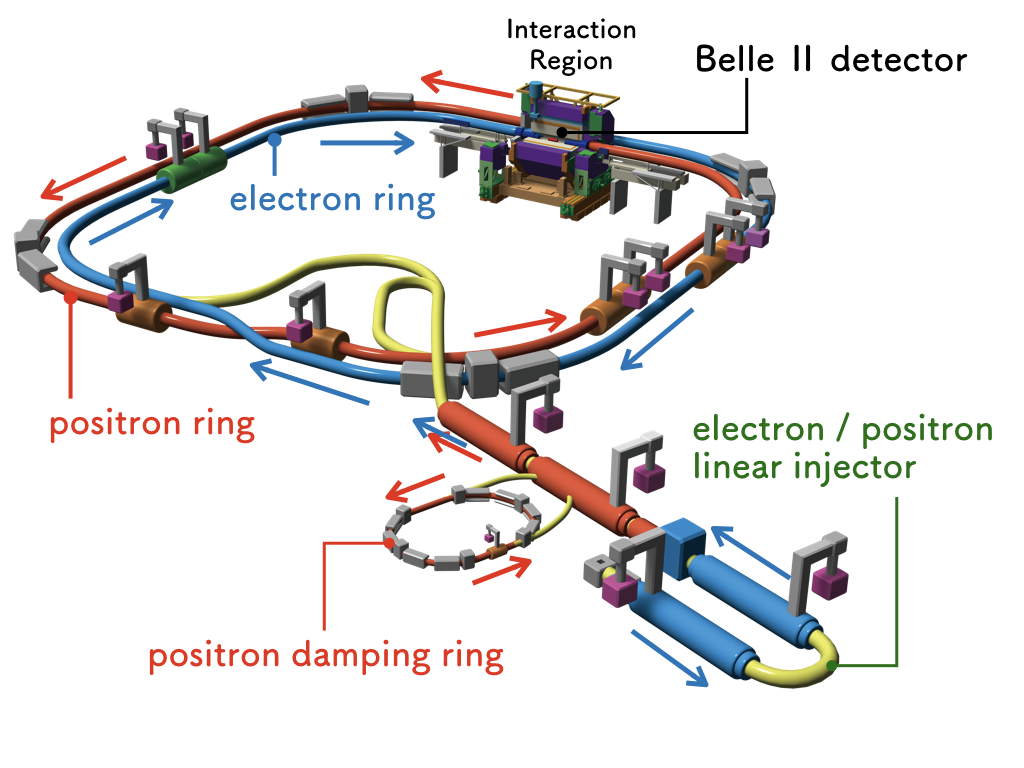
\includegraphics[width=0.8\textwidth]{./images/kek/layout_kekb.jpg}
    \caption{Schematic drawing of the accelerator complex at KEK~\cite{noauthor_operation_2024}.}
    \label{fig:kek:layout_superkekb}
\end{figure}

KEK is currently maintaining collaborations with several organizations, including CERN, to
facilitate research on various topics of interest. SuperKEKB is especially relevant to FCC-ee as it
can act as a prototype for testing innovative manufacturing, measurement, and analysis techniques,
whether in mechanical prototyping, elements alignment, or beam dynamics. During my secondment in
Japan, the optics measurement techniques utilized at CERN for the LHC, specifically turn-by-turn
acquisitions, were tested on the two rings of SuperKEKB. 
Previous studies have been conducted and are extended in this chapter. Rather than providing an
in-depth description, the focus here is on updating the previously employed techniques. For more
detailed information, please refer
to~\cite{keintzel_jacqueline_beam_2022,keintzel_superkekb_2021,keintzel_impact_2021}.


%=============================
%    Measurement Techniques
%=============================
\section{\review{Measurement Techniques for Linear Optics}}

In SuperKEKB, the beam optics are measured using either Closed Orbit
Distortion~\cite{ohnishi_optics_1999} or turn-by-turn measurements. As fast optics measurements can
be achieved with the TbT method, a measurement campaign has being carried out to improve the
measurement quality. This includes investigating various beam excitation techniques and settings.
The necessary pre-processing steps for optics measurements have been detailed
in~\cite{keintzel_jacqueline_beam_2022}, and are not covered here.


%------------------------------
%    Closed orbit distortion
%------------------------------
\subsection{\review{Closed Orbit Distortion}}

Optics measurements using the COD method
\cite{harrison_global_1987,chung_measurement_1993,ohnishi_optics_1999} are well established and
routinely performed at SuperKEKB. In COD measurements, the beam is excited using six corrector
magnets, and the centroid orbit is recorded by 466 BPMs for the HER and 444 BPMs for the LER,
respectively. The measured orbits, averaged over several turns, are stored in a matrix that contains
a large number of elements. The optics of both transverse planes are then reconstructed using
analytical formulas. Since the correctors must be powered one at a time, the COD method is
relatively time-consuming. 
Since the average particle orbit is observed, the BPM readings are highly dependent on precise
calibration. One significant advantage of COD measurements at SuperKEKB is that approximately 6.5
times more BPMs can be used compared to the TbT data.


%------------------------------
%        Turn-by-Turn
%------------------------------
\FloatBarrier
\subsection{\review{Turn-by-Turn}}

In SuperKEKB, 68 and 70 BPMs in the HER and LER rings are capable of recording turn-by-turn (TbT)
orbit data, typically capturing several thousand turns in both transverse planes. TbT measurements
are usually performed with a single bunch, with currents ranging from 0.2 mA to 1.5 mA. The beam can
be excited using three different methods.

First, an Injection Kicker (IK) delivers a single horizontal kick, causing the beam motion to damp
due to synchrotron radiation. The damping times for the positron and electron rings are 46 ms and 53
ms, corresponding to 4600 and 5300 turns, respectively~\cite{keintzel_jacqueline_beam_2022}.
However, the IK only provides horizontal kicks, limiting the precision of vertical optics
measurements.

In contrast, the Phase-Locked Loop (PLL) method allows continuous excitation of the beam and can
drive both horizontal and vertical planes. The PLL tracks the natural tune of the beam and drives it
at the corresponding frequency. A key advantage of the PLL system is that it can excite both planes
simultaneously, enabling measurements of transverse coupling and other resonance-driving terms
(RDTs). The PLL is currently the only method capable of performing vertical TbT measurements,
although data acquisition must be started manually, and a minimum bunch current of 0.5 mA is
required. This method was not used for the data discussed in this thesis.

The third method is not strictly an excitation. To induce oscillations in the vertical plane, the 
beam can be injected with an orbit offset. This vertical offset causes the beam to oscillate as if 
it had received a single kick. The oscillations then damp, and a new beam must be injected to repeat 
the measurement. This method has been successfully used for the first time to measure vertical
optics using turn-by-turn data.

Once the TbT data is recorded, the standard analysis procedures outlined in
\cref{section:opticcs_meas} are applied. Specifically, the frequency spectrum is calculated before
reconstructing the optics. The model used for this analysis is generated with the SAD (Strategic
Accelerator Design) software \cite{noauthor_sad_nodate}.
A typical turn-by-turn signal is depicted in \cref{fig:kek:tbt_signal}.


\begin{figure}[!htb]
    \centering
    \begin{subfigure}[c]{0.47\textwidth}
        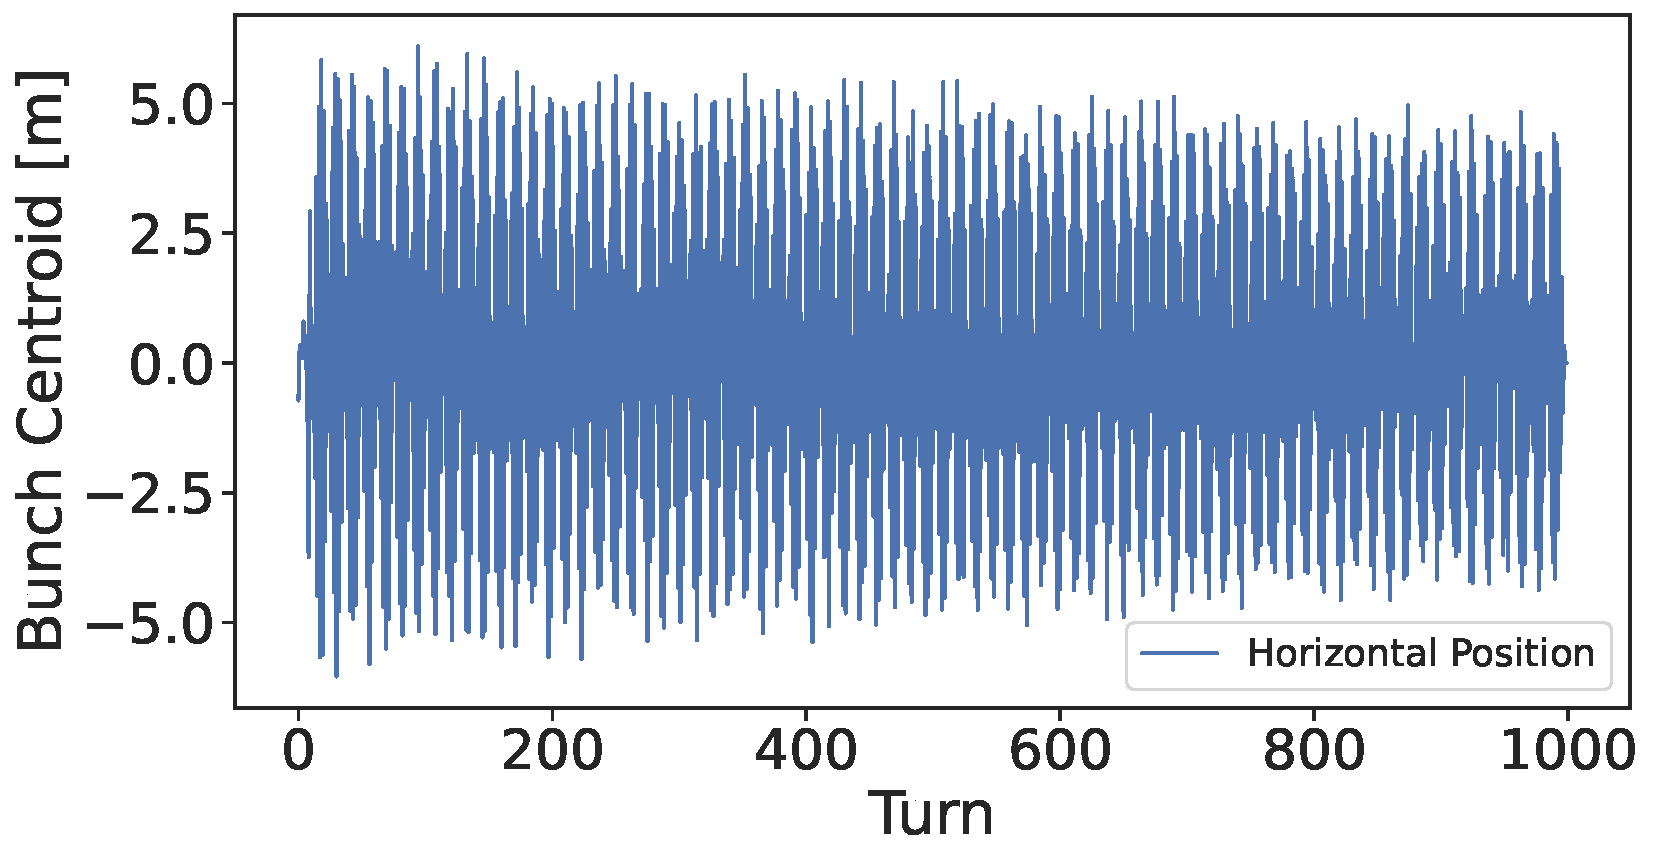
\includegraphics[width=\linewidth]{images/kek/horizontal_tbt_ler.pdf}
        \caption{Horizontal plane, oscillations are created by the Injection Kicker.}
    \end{subfigure}
    \hfill
    \begin{subfigure}[c]{0.48\textwidth}
        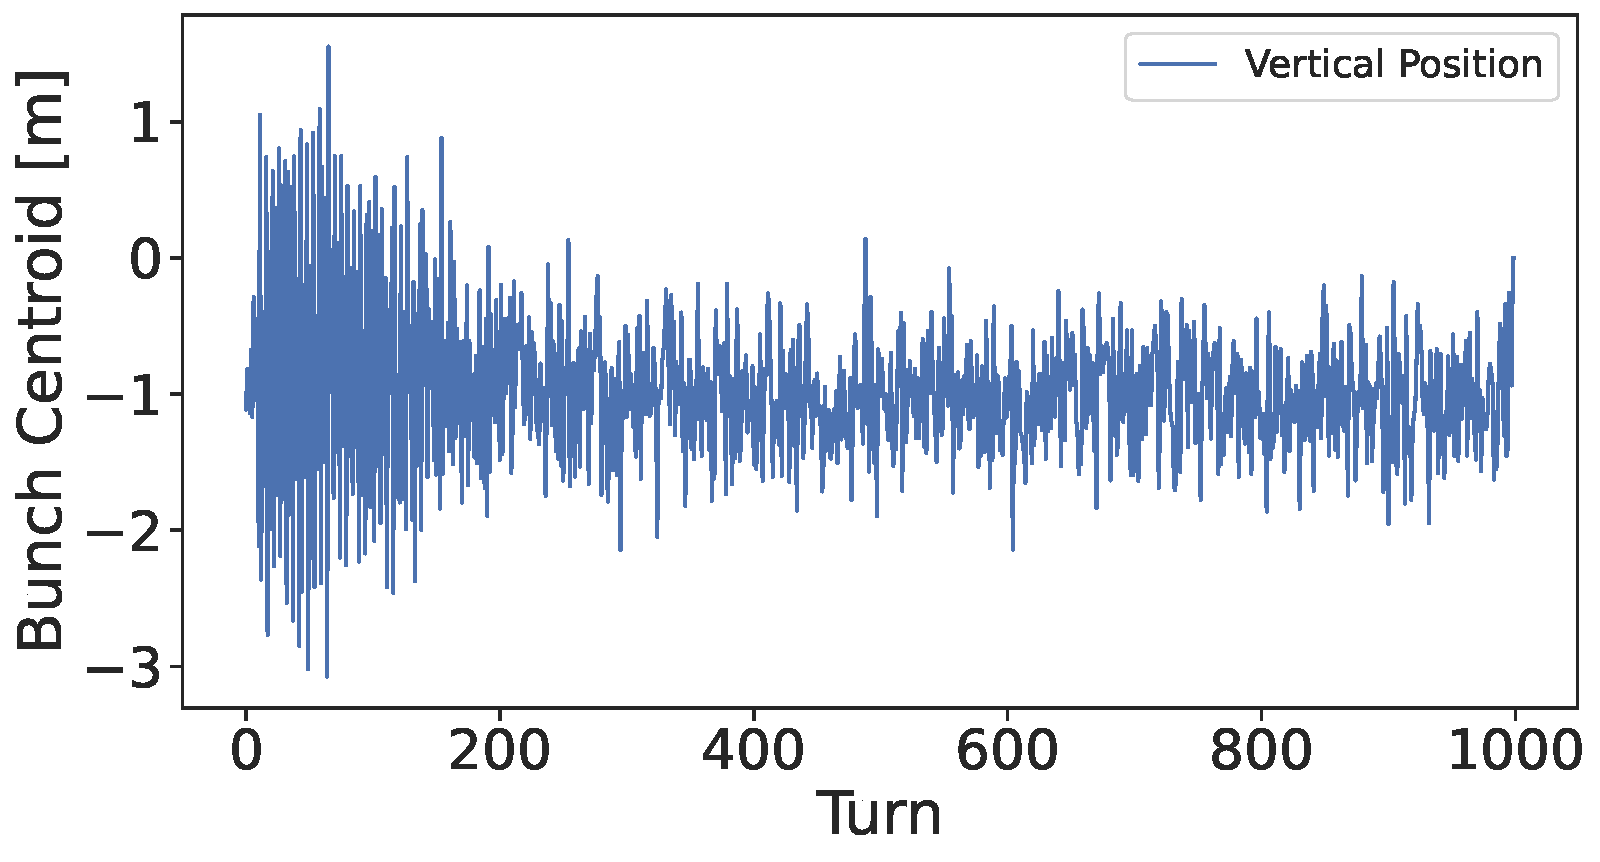
\includegraphics[width=\linewidth]{images/kek/vertical_tbt_ler.pdf}
        \caption{Vertical plane, oscillations are created via an injection offset.}
    \end{subfigure}
    \caption{Typical horizontal and vertical recorded turn-by-turn signal.}
    \label{fig:kek:tbt_signal}
\end{figure}



%------------------------------
%            GUI
%------------------------------
\subsection{\review{OMC3 Graphical User Interface}}

The graphical user interface (GUI) used for optics analysis on the LHC, based on OMC3
\cite{omc-team_omc3_2021}, has been updated to support the HER and LER rings of SuperKEKB. This tool
is essential for the rapid and efficient cleaning of bad kicks, BPMs, and for detecting resonance
lines. Utilizing the latest version of the GUI provides access to recent bug fixes and improvements,
enhancing usability and functionality. A typical use case is illustrated in
\cref{fig:kek:gui_bad_bpms}, where BPMs that provide erroneous data across multiple measurements can
be easily identified.

\begin{figure}[!htb]
    \centering
    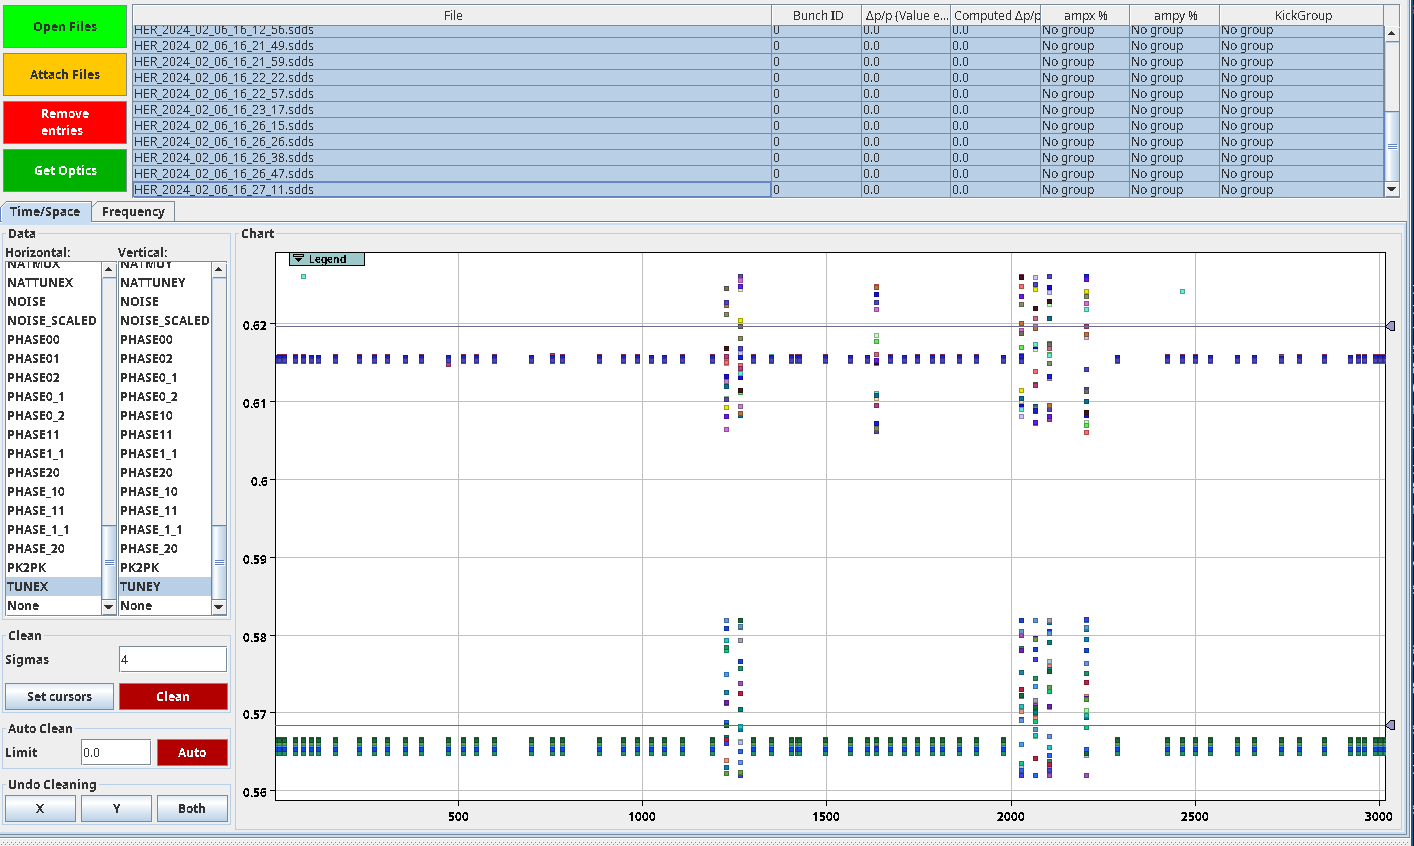
\includegraphics[width=0.8\textwidth]{./images/kek/GUIbadbpm.png}
    \caption{The identification of bad BPMs across measurements is easily done with the GUI.}
    \label{fig:kek:gui_bad_bpms}
\end{figure}



%=============================
%     Optics Observations
%=============================
\FloatBarrier
\section{\todo{Optics Observations}}

All the measurements presented in this section have been performed in February 2024, during the
commissioning phase of SuperKEKB.

%-----------------------------
%        Turn-by-Turn
%-----------------------------
\subsection{\todo{Beta-Beating}}

Several configurations of the machine were measured using turn-by-turn acquisitions, as detailed in
\cref{tab:superkekb:configurations}. The configurations with $\beta_y^* = 48.6$ in LER and
$\beta_y^* = 81$ in HER are referred to as \textit{detuned}. Multiple kicks were performed for each
configuration to increase measurement precision. Although additional measurements were taken,
insufficient kick amplitude in some cases made it challenging to extract reliable linear optics
data and are thus here not included. Specifically, vertical measurements are challenging to perform
as oscillation amplitudes are often low due to the limited achievable offset.
Overall, both the \textit{detuned} and \text{8mm squeezed} optics have been reliably measured for
both rings. However, vertical measurements for the squeezed optics are still challenging to measure 
in LER.

\begin{table}
    \centering
    \begin{tabular}{llrrrrr}
    \hline
    Ring & Day & $\beta_x^*$ [mm] & $\beta_y^*$ [mm] & $Q_x$ & $Q_y$ & Kicks\\
    \hline
    LER        & 06 & 384 &\textbf{48.6} & 44.556 & 46.635 & H \& V \\
               & 09 & 384 &\textbf{48.6} & 44.553 & 46.621 & H  \\
               \hdashline
               & 20 & 200 & \textbf{8}   & 44.527 & 46.604 & H \\
               & 22 & 200 & \textbf{8}   & 44.535 & 46.590 & H \\
               &&&&&& \\
    HER        & 06 & 400 & \textbf{81}  & 45.572 & 43.616 & H \& V\\
               \hdashline
               & 20 & 200 & \textbf{8} & 45.530 & 43.595 & H \\
               & 22 & 200 & \textbf{8} & 45.535 & 43.596 & V \\
               & 26 & 200 & \textbf{8} & 45.535 & 43.596 & V \\
    \bottomrule
    \end{tabular}
  \caption{Configurations of the HER and LER rings for measurements performed via turn-by-turn
  acquisition.}
  \label{tab:superkekb:configurations}
\end{table}


%-----------------------------
%            LER 
\FloatBarrier
\subsubsection{\todo{LER $\beta-beating$}}

\begin{figure}[!htb]
    \centering
    \begin{subfigure}[b]{0.48\textwidth}
        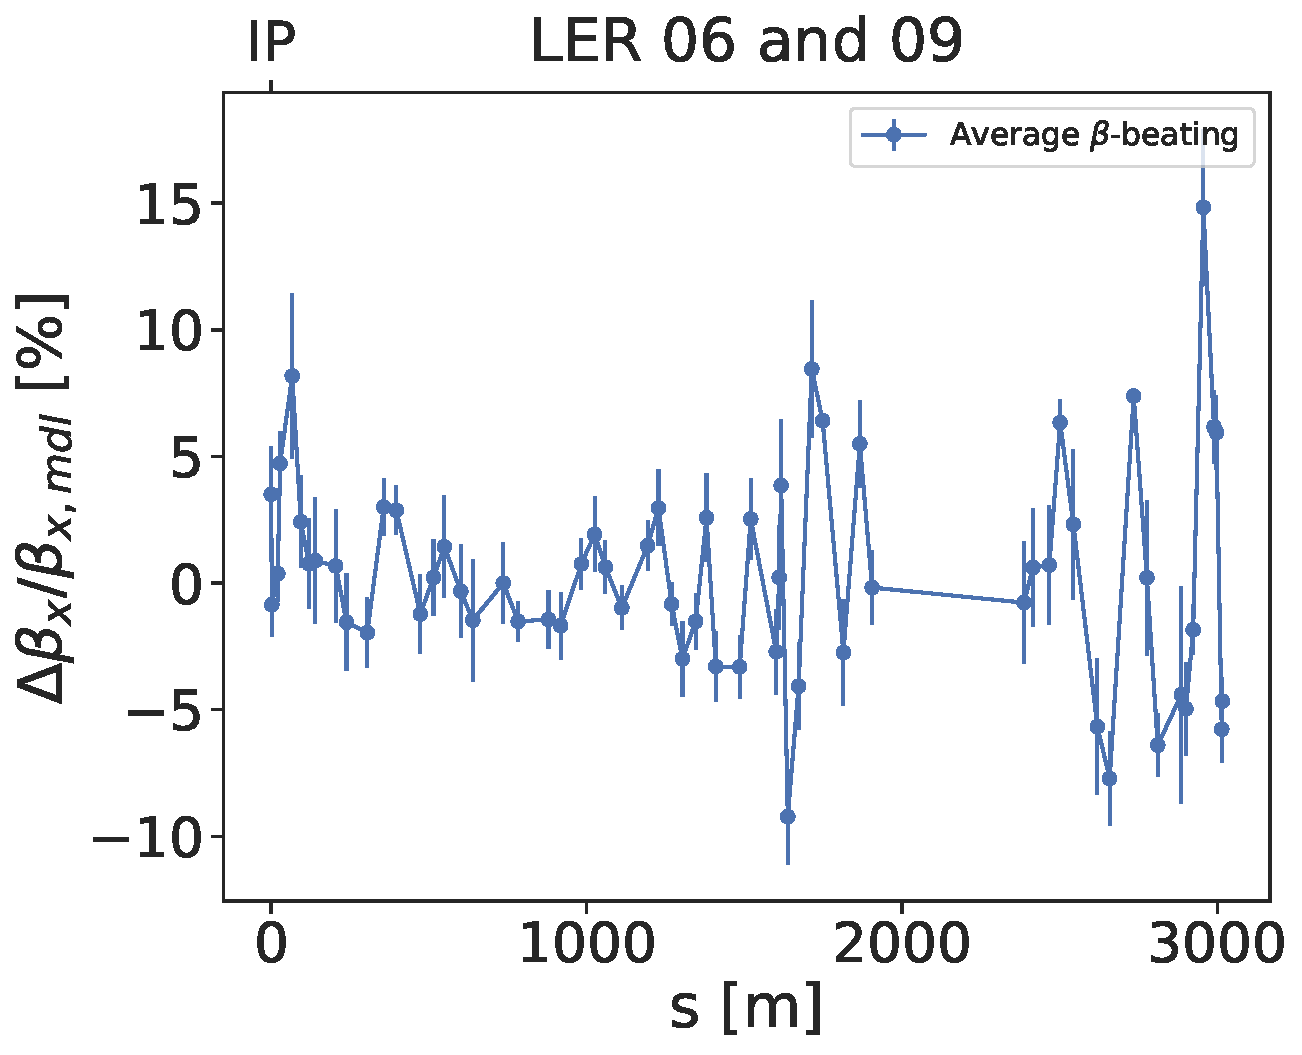
\includegraphics[width=\linewidth]{images/kek/ler_06_09_bet_x.pdf}
        \caption{Horizontal beta-beating, RMS is $\approx 4\%$.}
    \end{subfigure}
    \hfill
    \begin{subfigure}[b]{0.48\textwidth}
        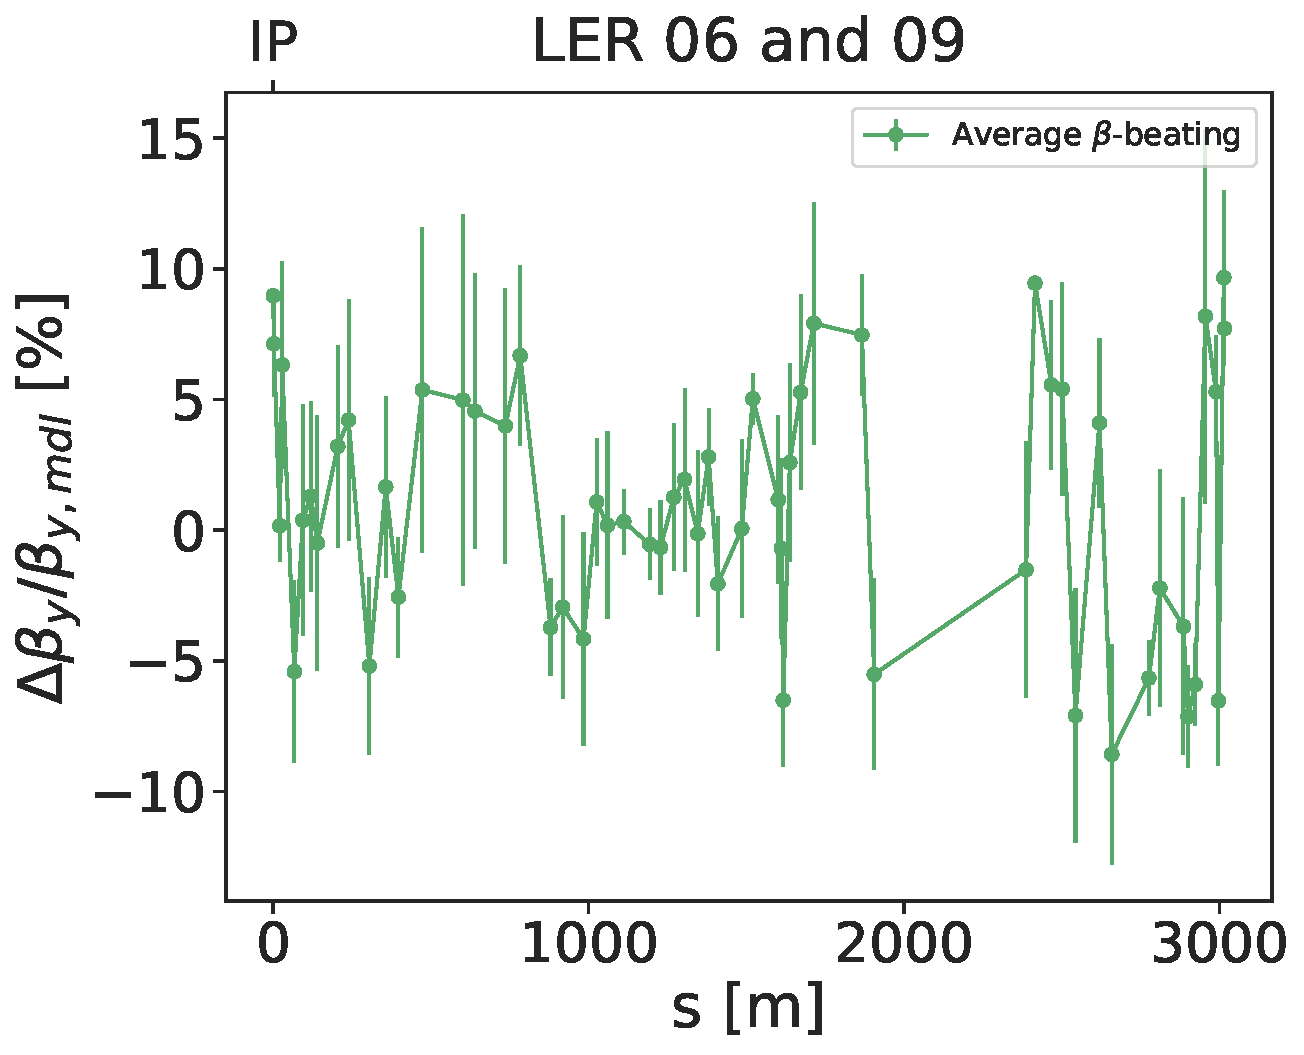
\includegraphics[width=\linewidth]{images/kek/ler_06_09_bet_y.pdf}
        \caption{Vertical beta-beating, RMS is $\approx 4\%$.}
    \end{subfigure}
    \caption{LER horizontal and vertical beta-beating for \textit{detuned} optics, reliably measured
    during two different days.  The vertical plane is noticeably noisier as oscillation amplitudes
    are smaller.}
    \label{fig:kek:beating_ler_detuned}
\end{figure}

action 5 times lower than horizontal

\begin{figure}[!htb]
    \centering
    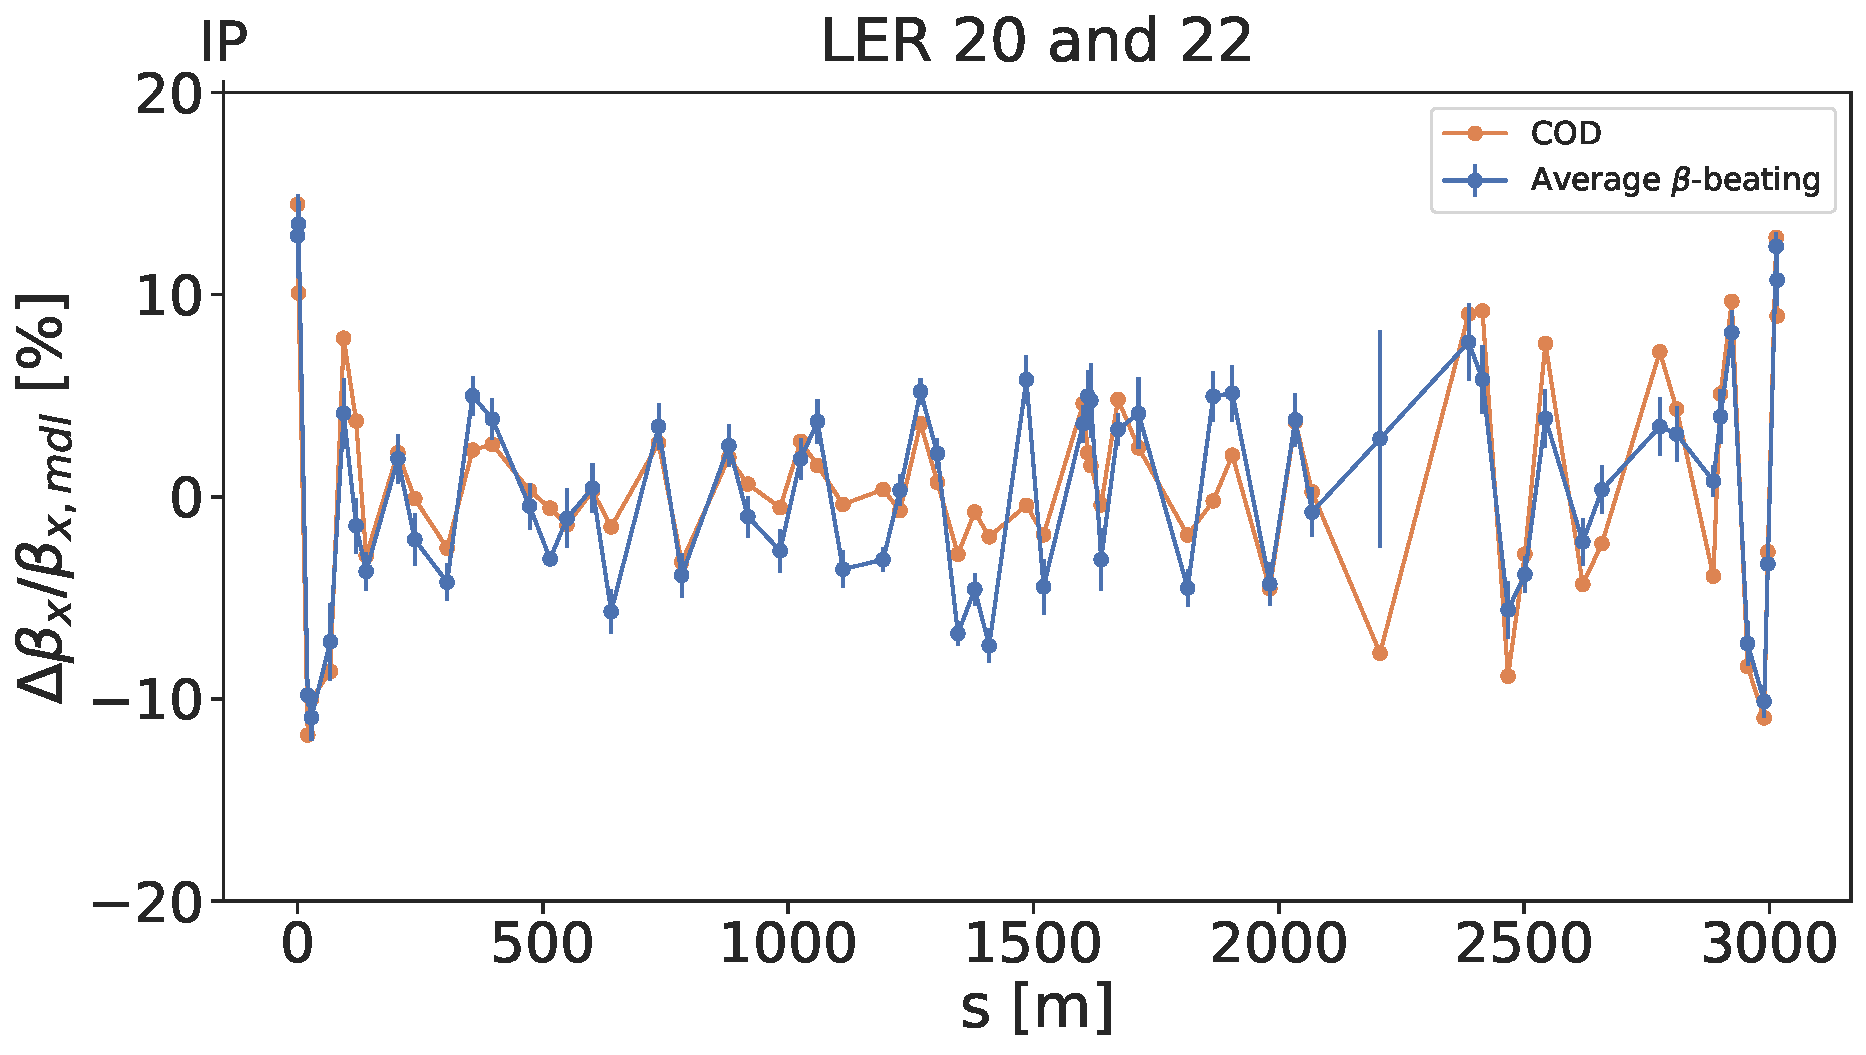
\includegraphics[width=0.7\linewidth]{images/kek/ler_20_22_bet_x.pdf}
    \caption{LER horizontal beta-beating for \textit{8mm squeezed} optics, reliably measured during
    two different days. The vertical plane is absent due to amplitudes being too low to reconstruct
    linear optics. A comparison to the beating measured via COD is made.}
    \label{fig:kek:beating_ler_squeezed}
\end{figure}



%-----------------------------
%            HER
\FloatBarrier
\subsubsection{\todo{HER $\beta-beating$}}

\begin{figure}[!htb]
    \centering
    \begin{subfigure}[b]{0.48\textwidth}
        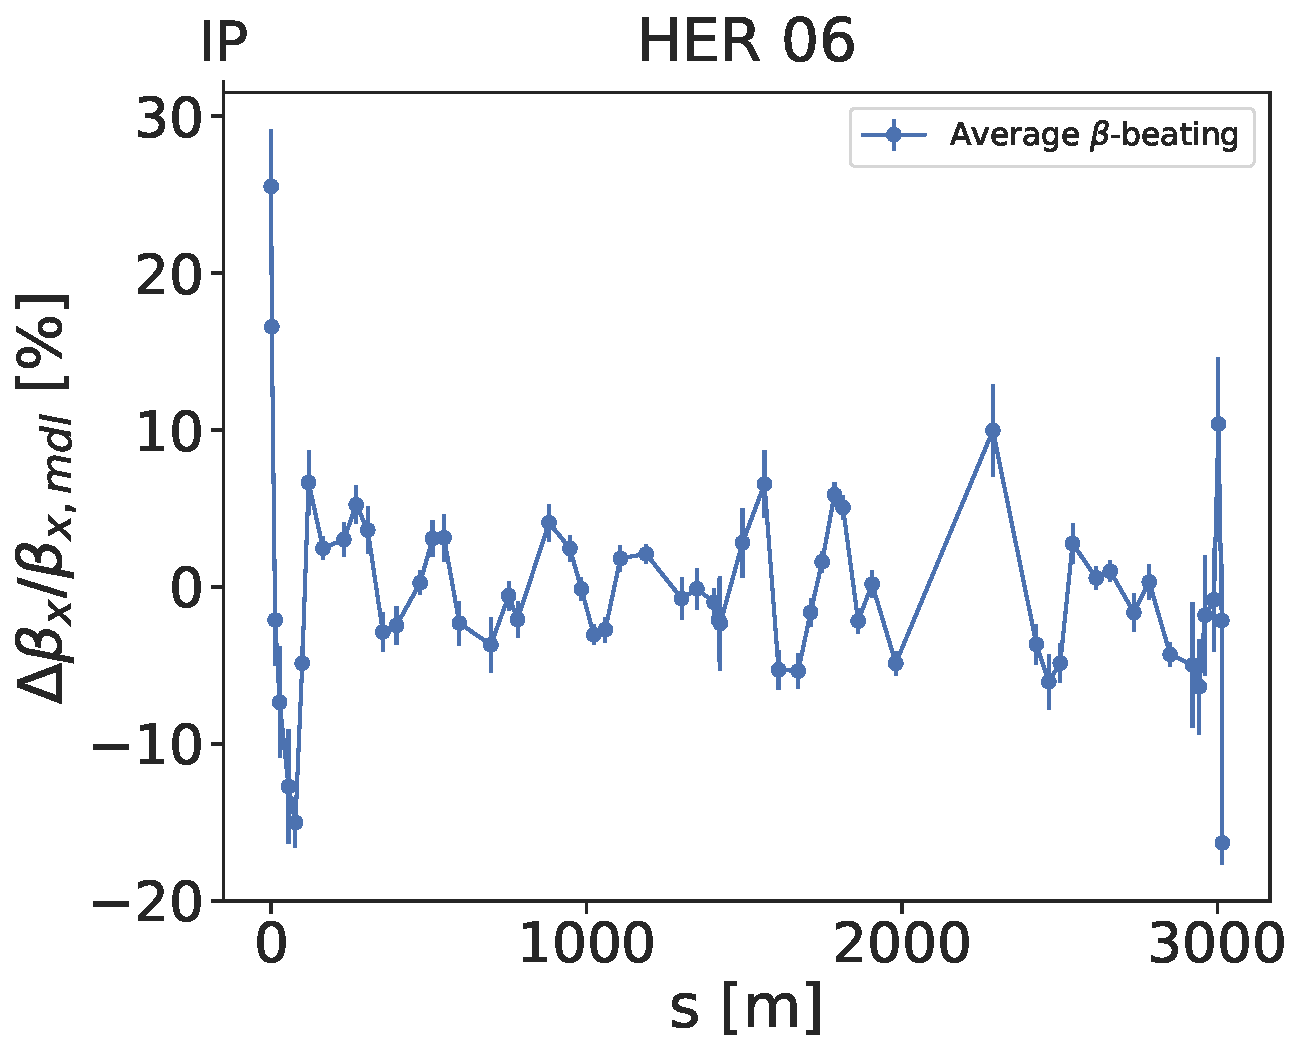
\includegraphics[width=\linewidth]{images/kek/her_06_bet_x.pdf}
        \caption{Horizontal beta-beating, RMS is $\approx 6\%$.}
    \end{subfigure}
    \hfill
    \begin{subfigure}[b]{0.48\textwidth}
        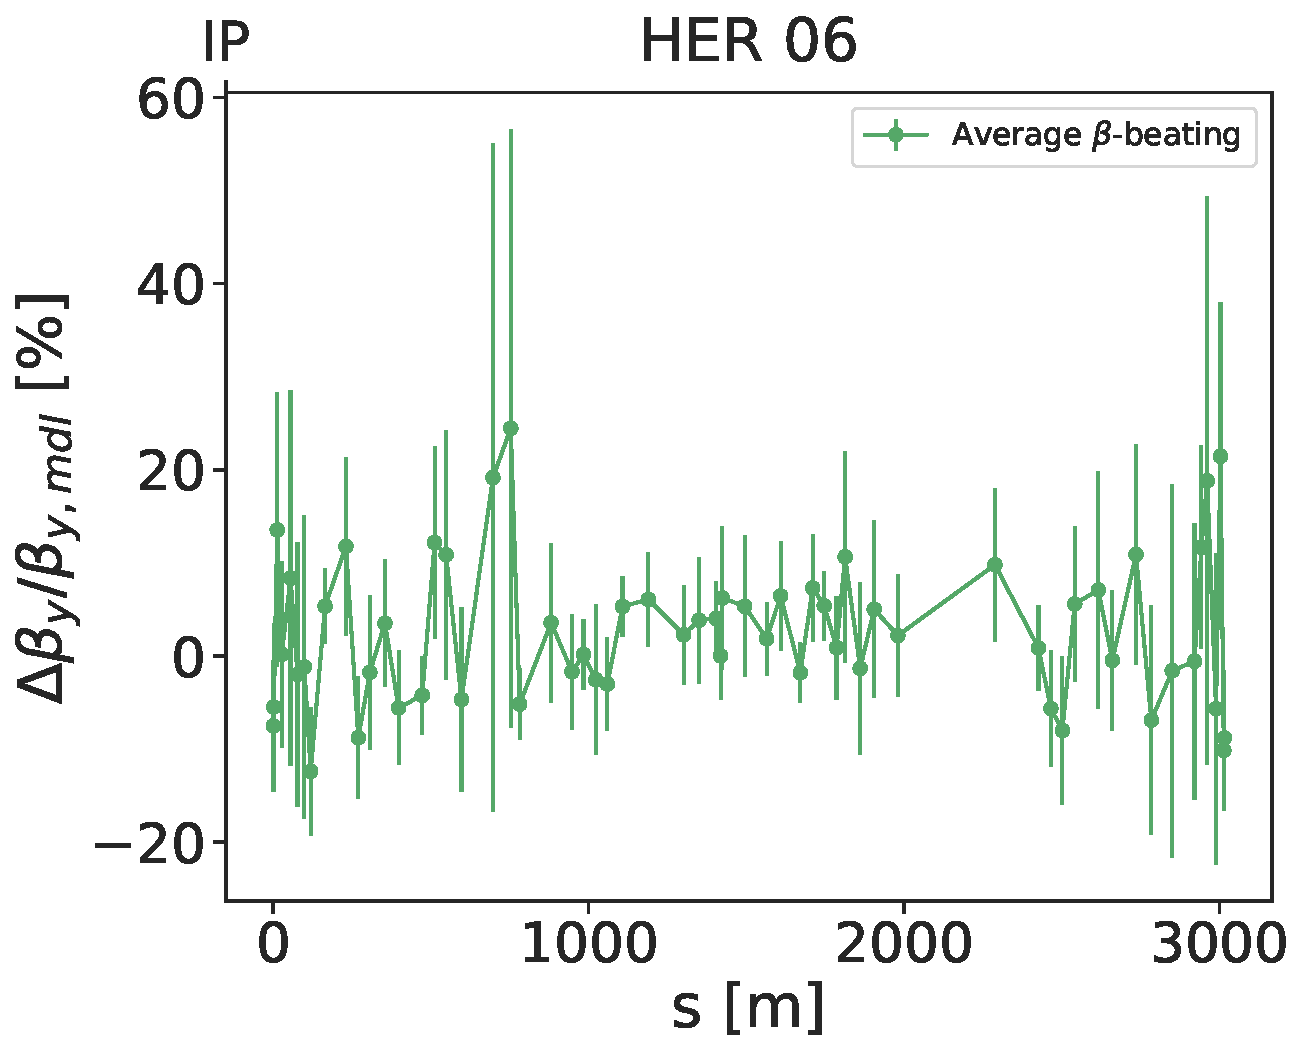
\includegraphics[width=\linewidth]{images/kek/her_06_bet_y.pdf}
        \caption{Vertical beta-beating, RMS is $\approx 8\%$.}
    \end{subfigure}
    \caption{HER horizontal and vertical beta-beating for \textit{detuned} optics. The vertical
    plane is noticeably noisier as oscillation amplitudes are smaller.}
    \label{fig:kek:beating_her_detuned}
\end{figure}

action 5 times lower than H

\begin{figure}[!htb]
    \centering
    \begin{subfigure}[b]{0.48\textwidth}
        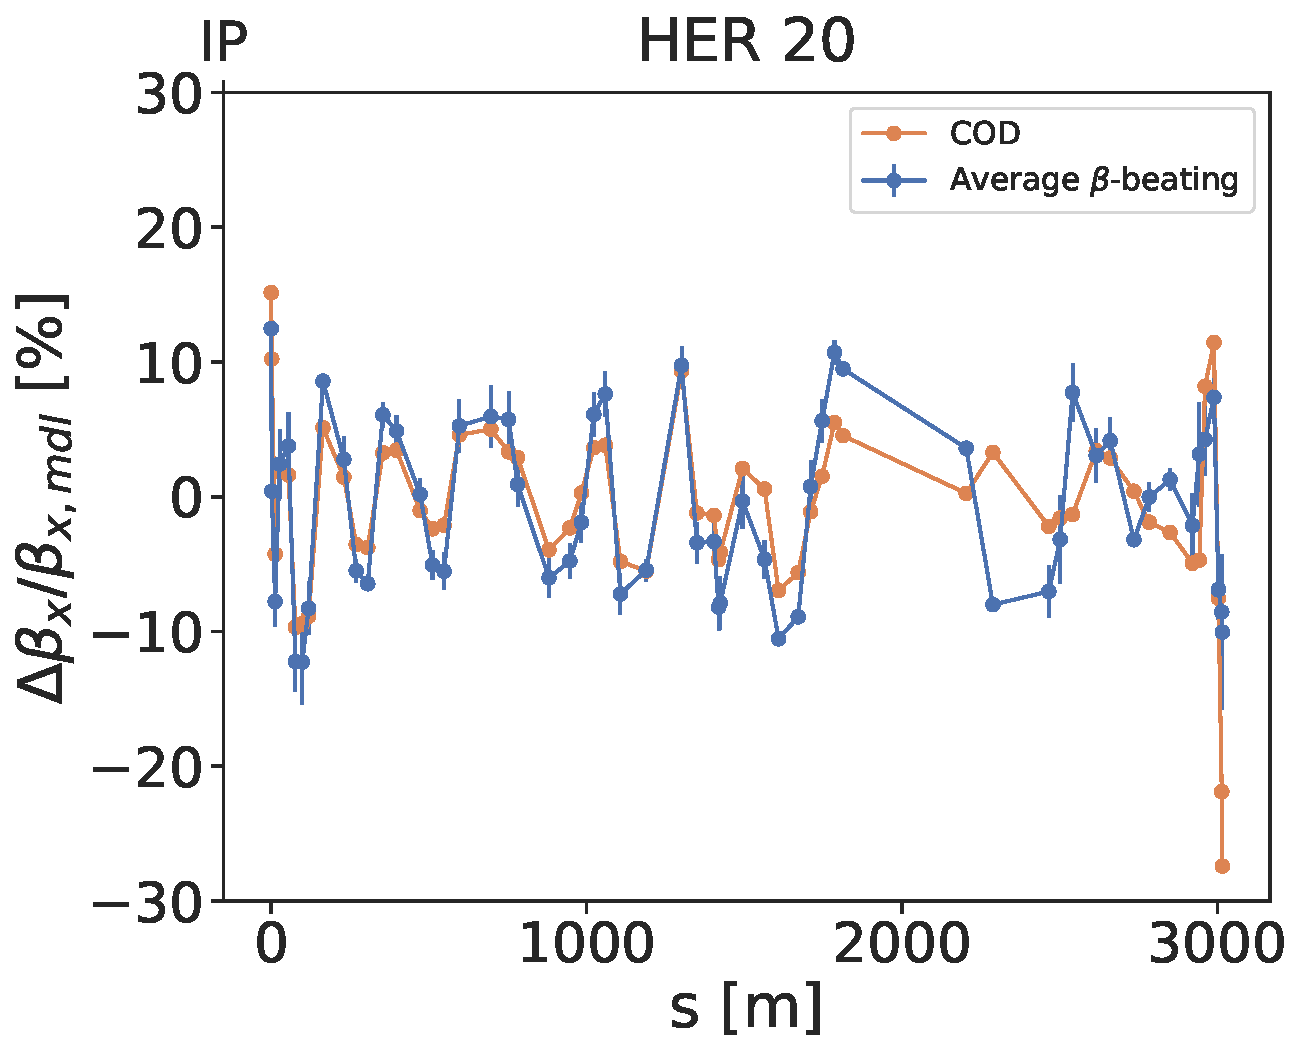
\includegraphics[width=\linewidth]{images/kek/her_20_bet_x_unzoomed.pdf}
        \caption{Horizontal beta-beating, RMS is $\approx 7\%$.}
    \end{subfigure}
    \hfill
    \begin{subfigure}[b]{0.48\textwidth}
        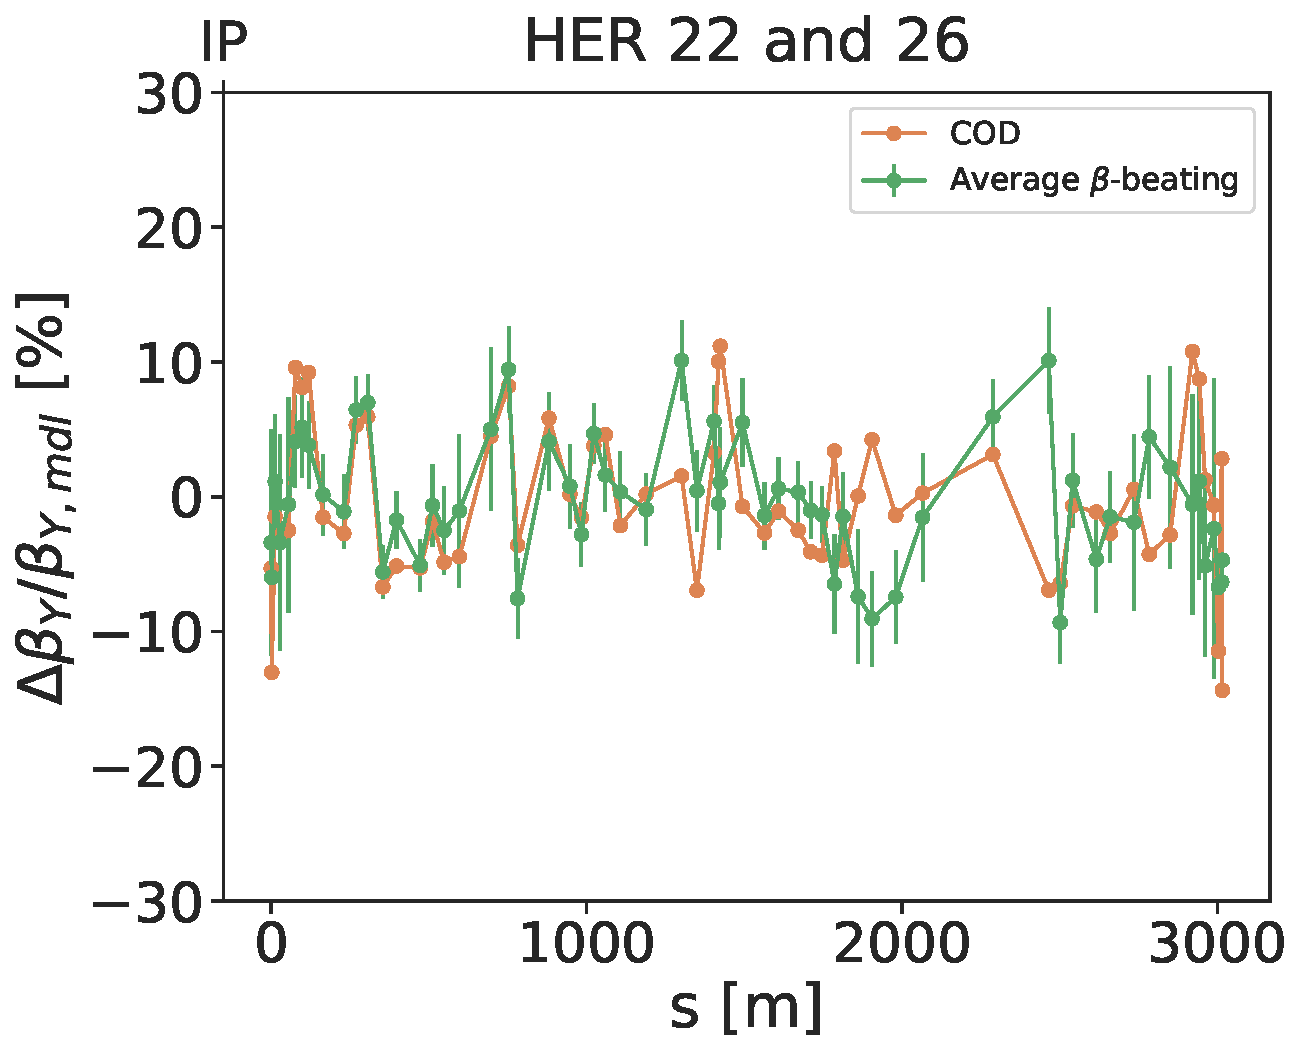
\includegraphics[width=\linewidth]{images/kek/her_22_26_bet_y_unzoomed.pdf}
        \caption{Vertical beta-beating, RMS is $\approx 5\%$.}
    \end{subfigure}
    \caption{HER horizontal and vertical beta-beating for \textit{8mm squeezed} optics. The vertical
    plane is noticeably noisier as oscillation amplitudes are smaller. A comparison to the beating
    measured via COD is made.}
    \label{fig:kek:beating_her_squeezed}
\end{figure}



%-----------------------------
%            Summary
\FloatBarrier
\subsubsection{\todo{Summary}}

\begin{table}
    \centering
    \begin{tabular}{llrr}
        \toprule
        Ring & Configuration & $\beta$-b. rms H & $\beta$-b. rms V \\
        \midrule
        LER  &  Detuned      & 4\%              & 5\%   \\
            &  Squeezed 8mm & 6\%              &       \\
        HER  &  Detuned      & 6\%              & 8\%  \\
            &  Squeezed 8mm & 7\%              & 5\%  \\
        \bottomrule
    \end{tabular}
    \caption{Summary of the measured $\beta$-beating with squeezed and detuned optics in the HER
    and LER rings.}
    \label{tab:kek:summary_beating}
\end{table}



%-----------------------------
%         LER Amp.Det.
%-----------------------------
\FloatBarrier
\subsection{\review{Amplitude Detuning}}

%-----------------------------
%         Tune Stability
\FloatBarrier
\subsubsection{\review{Tune Stability}}

To accurately measure non-linear optics, reliable measurement of the tune is essential. Ensuring
tune stability across consecutive kicks is needed to minimize measurement uncertainties and reflects
the reproducibility of the machine. With an appropriate kicker in the horizontal plane, this plane
is expected to be easier to measure, and is reflected by the tune stability accross kicks.
\Cref{fig:kek:shots} illustrates the variation in tune from the first kick compared to subsequent
kicks for both rings and planes.
While reproducibility is challenging to achieve in the vertical plane of the LER, all other
measurements agree well together, down to a few tune units of $10^{-3}$.

\begin{figure}[!htb]
    \centering
    \begin{subfigure}[b]{0.48\textwidth}
        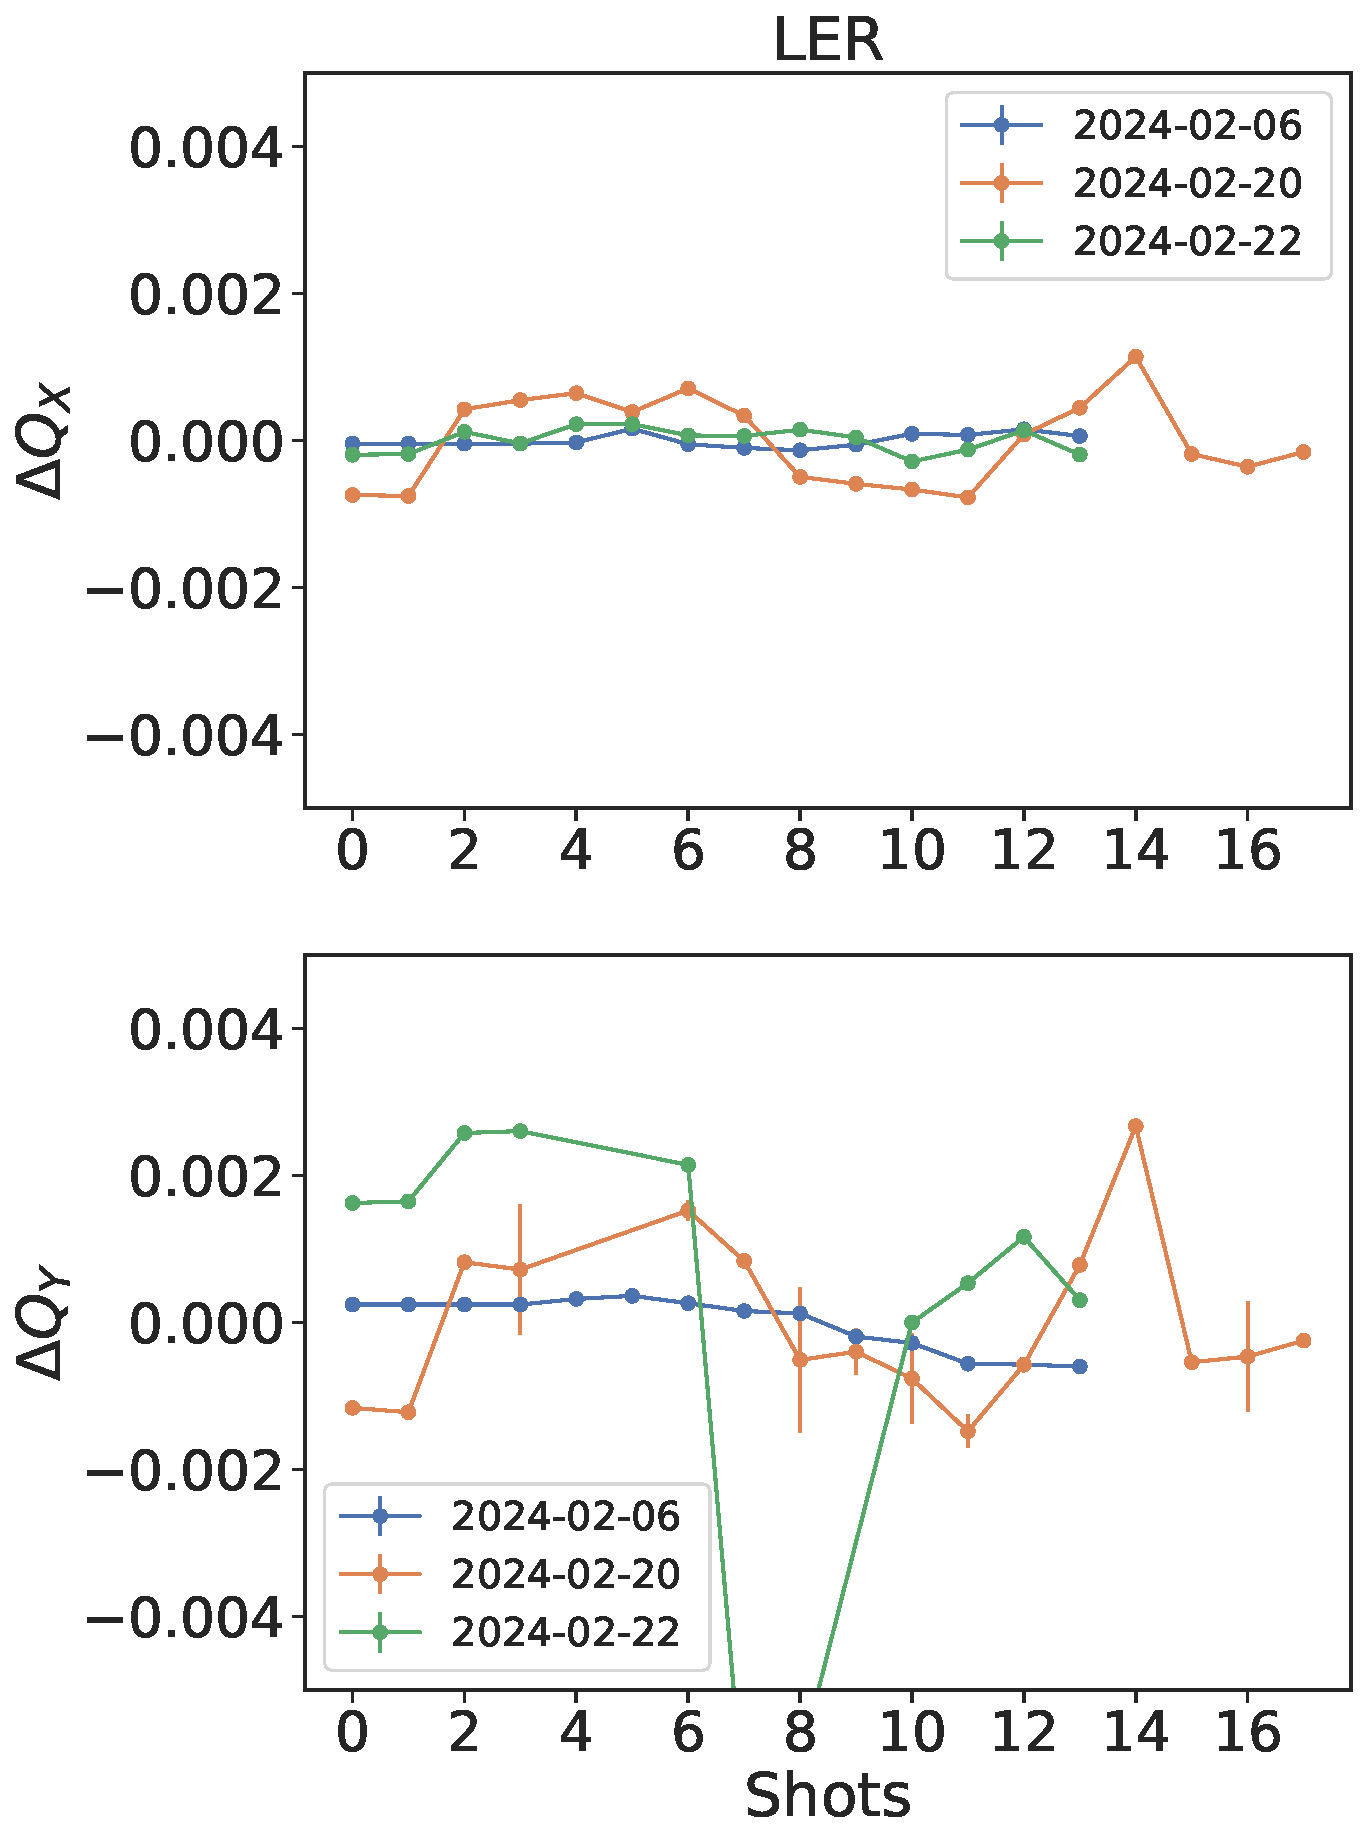
\includegraphics[width=\linewidth]{images/kek/SUPERKEKBLER_shots.pdf}
        \caption{Tune stability for the LER ring.}
    \end{subfigure}
    \hfill
    \begin{subfigure}[b]{0.48\textwidth}
        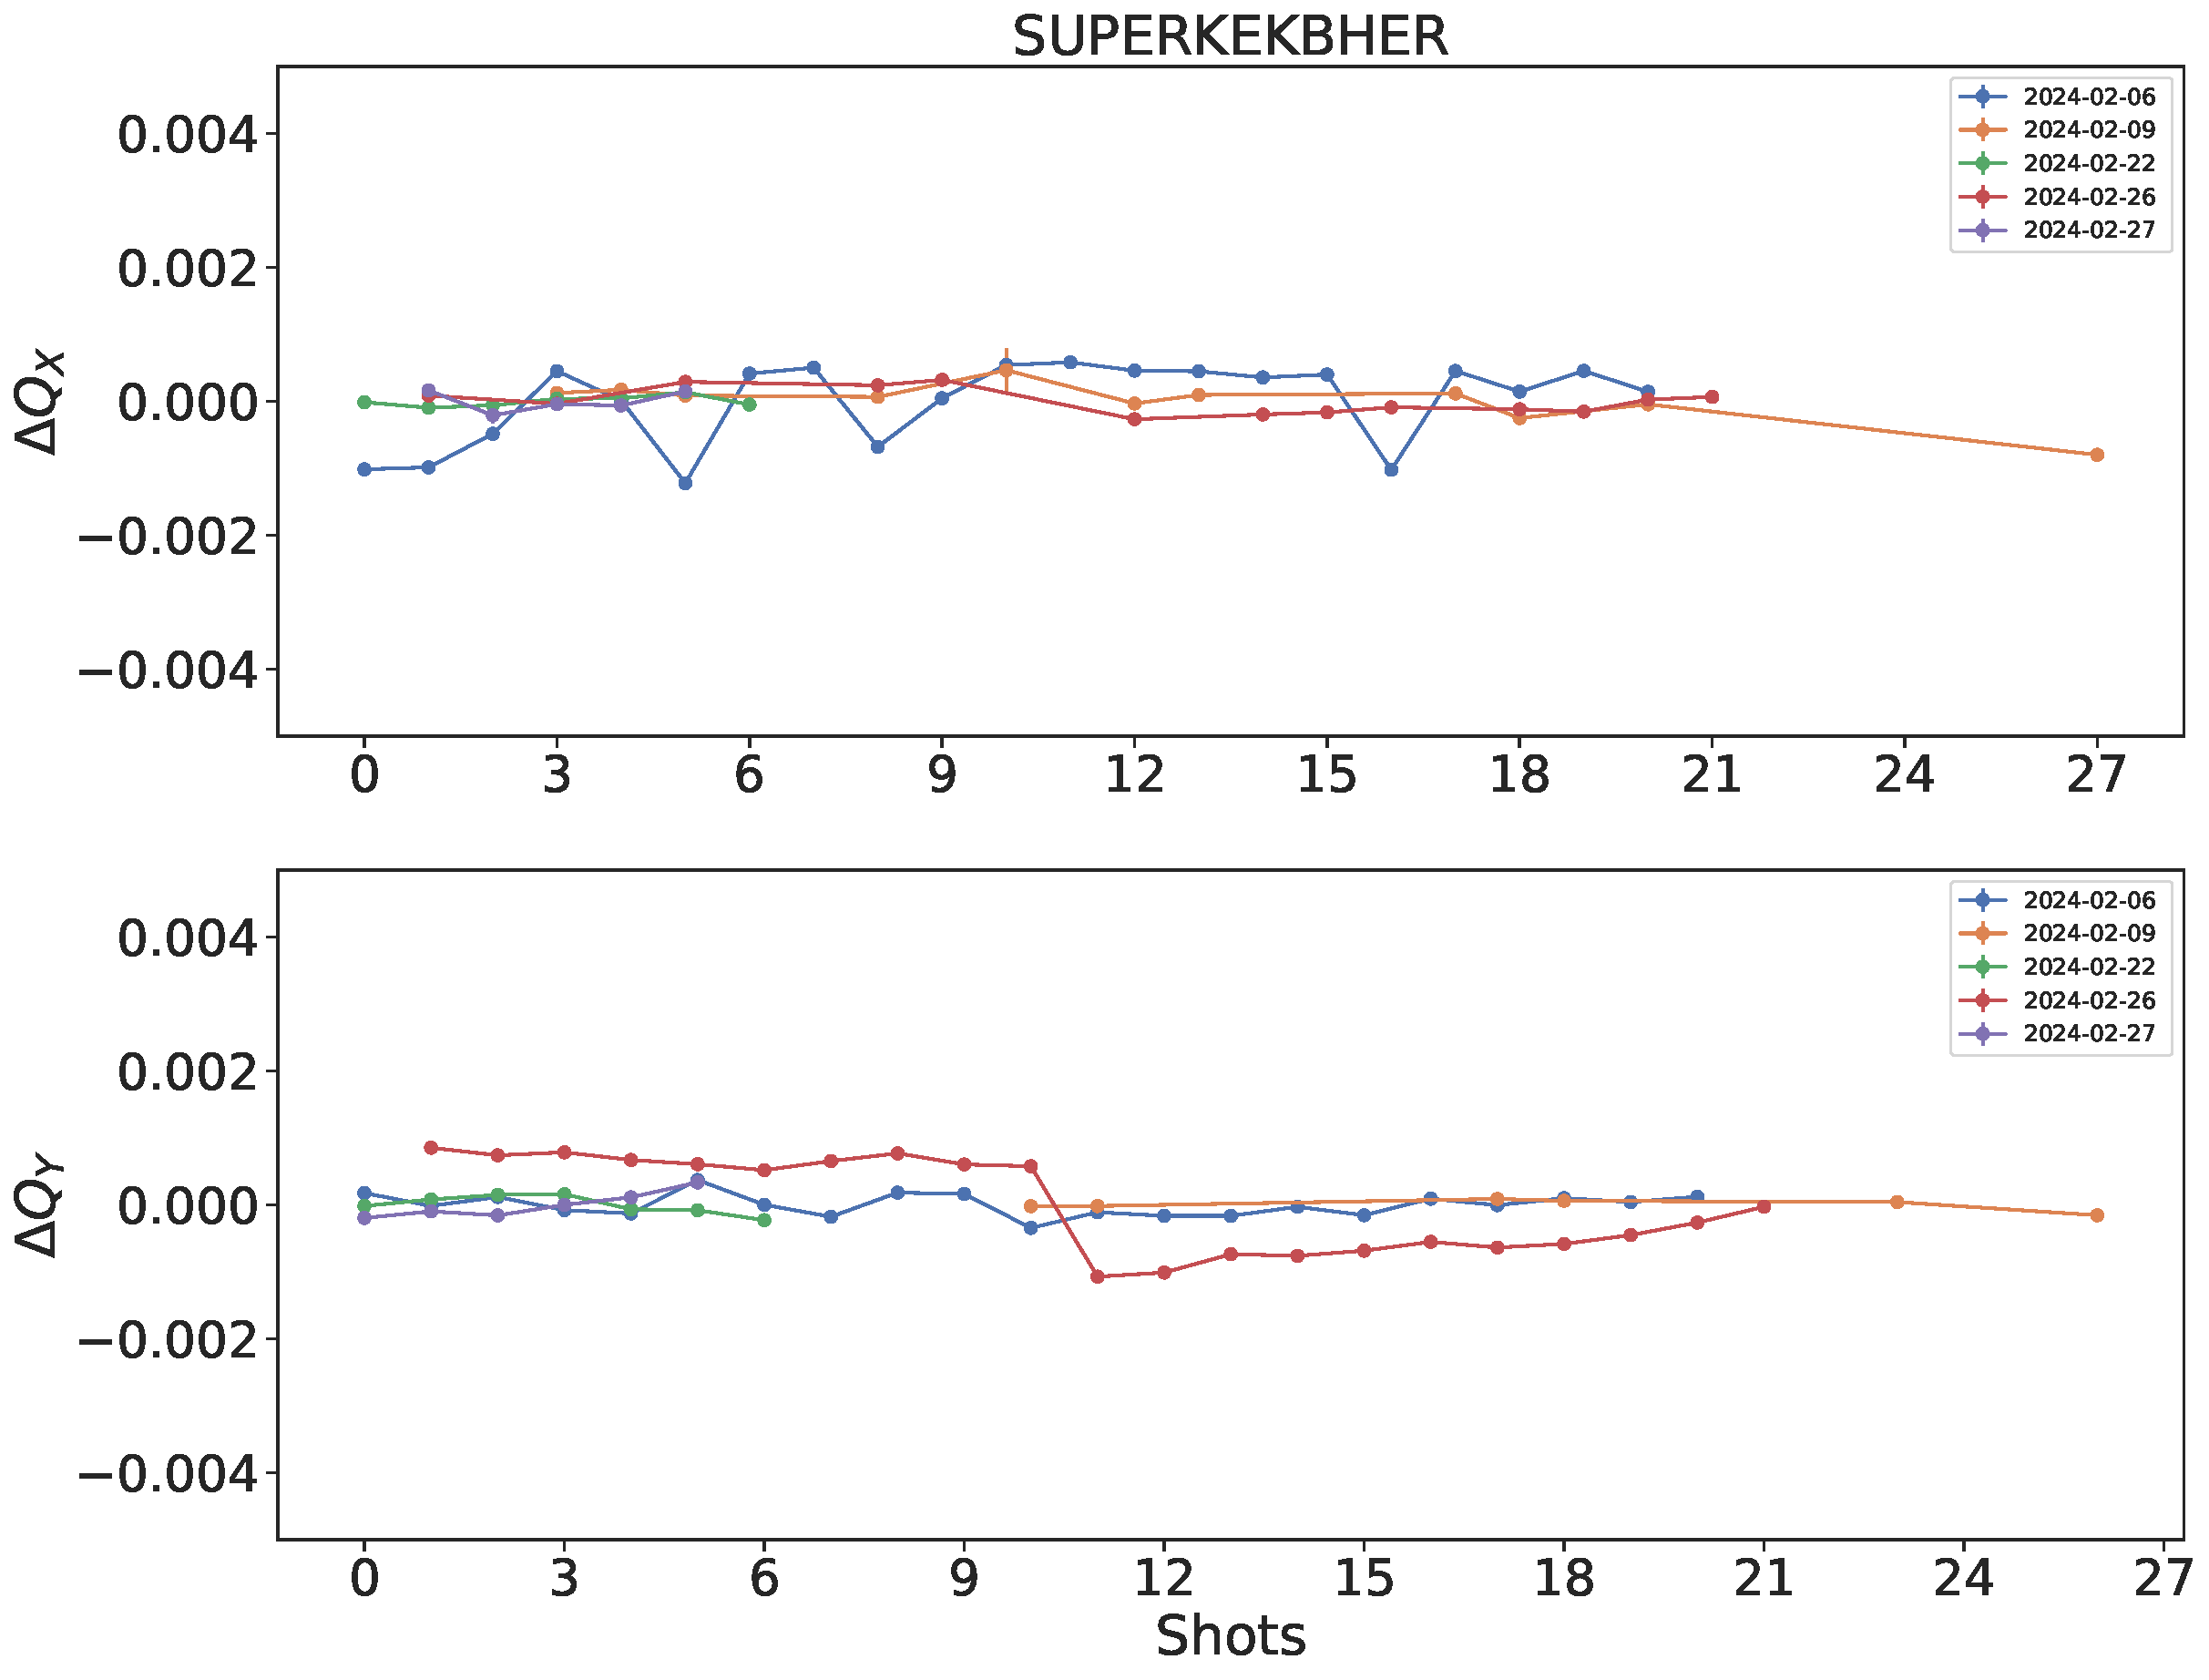
\includegraphics[width=\linewidth]{images/kek/SUPERKEKBHER_shots.pdf}
        \caption{Tune stability for the HER ring.}
    \end{subfigure}
    \caption{Difference in tune between consecutive measurements, across several days.}
    \label{fig:kek:shots}
\end{figure}


%-----------------------------
%             LER
\FloatBarrier
\subsubsection{\review{Amplitude Detuning in LER}}

Particularly notable measurements have been conducted in the LER ring with \textit{detuned} optics.
These measurements stand out due to their larger action range compared to others.
\Cref{fig:kek:ler_full_tune_ampdet} illustrates the various kicks performed and their corresponding
action.
The tune is computed across each kick using a window of 200 turns, every 50 turns. A clear trend is
emerges with the tune following the amplitude of the kicks. Over time, the oscillations gradually
dampen, and the tune changes accordingly.

\begin{figure}[!htb]
    \centering
    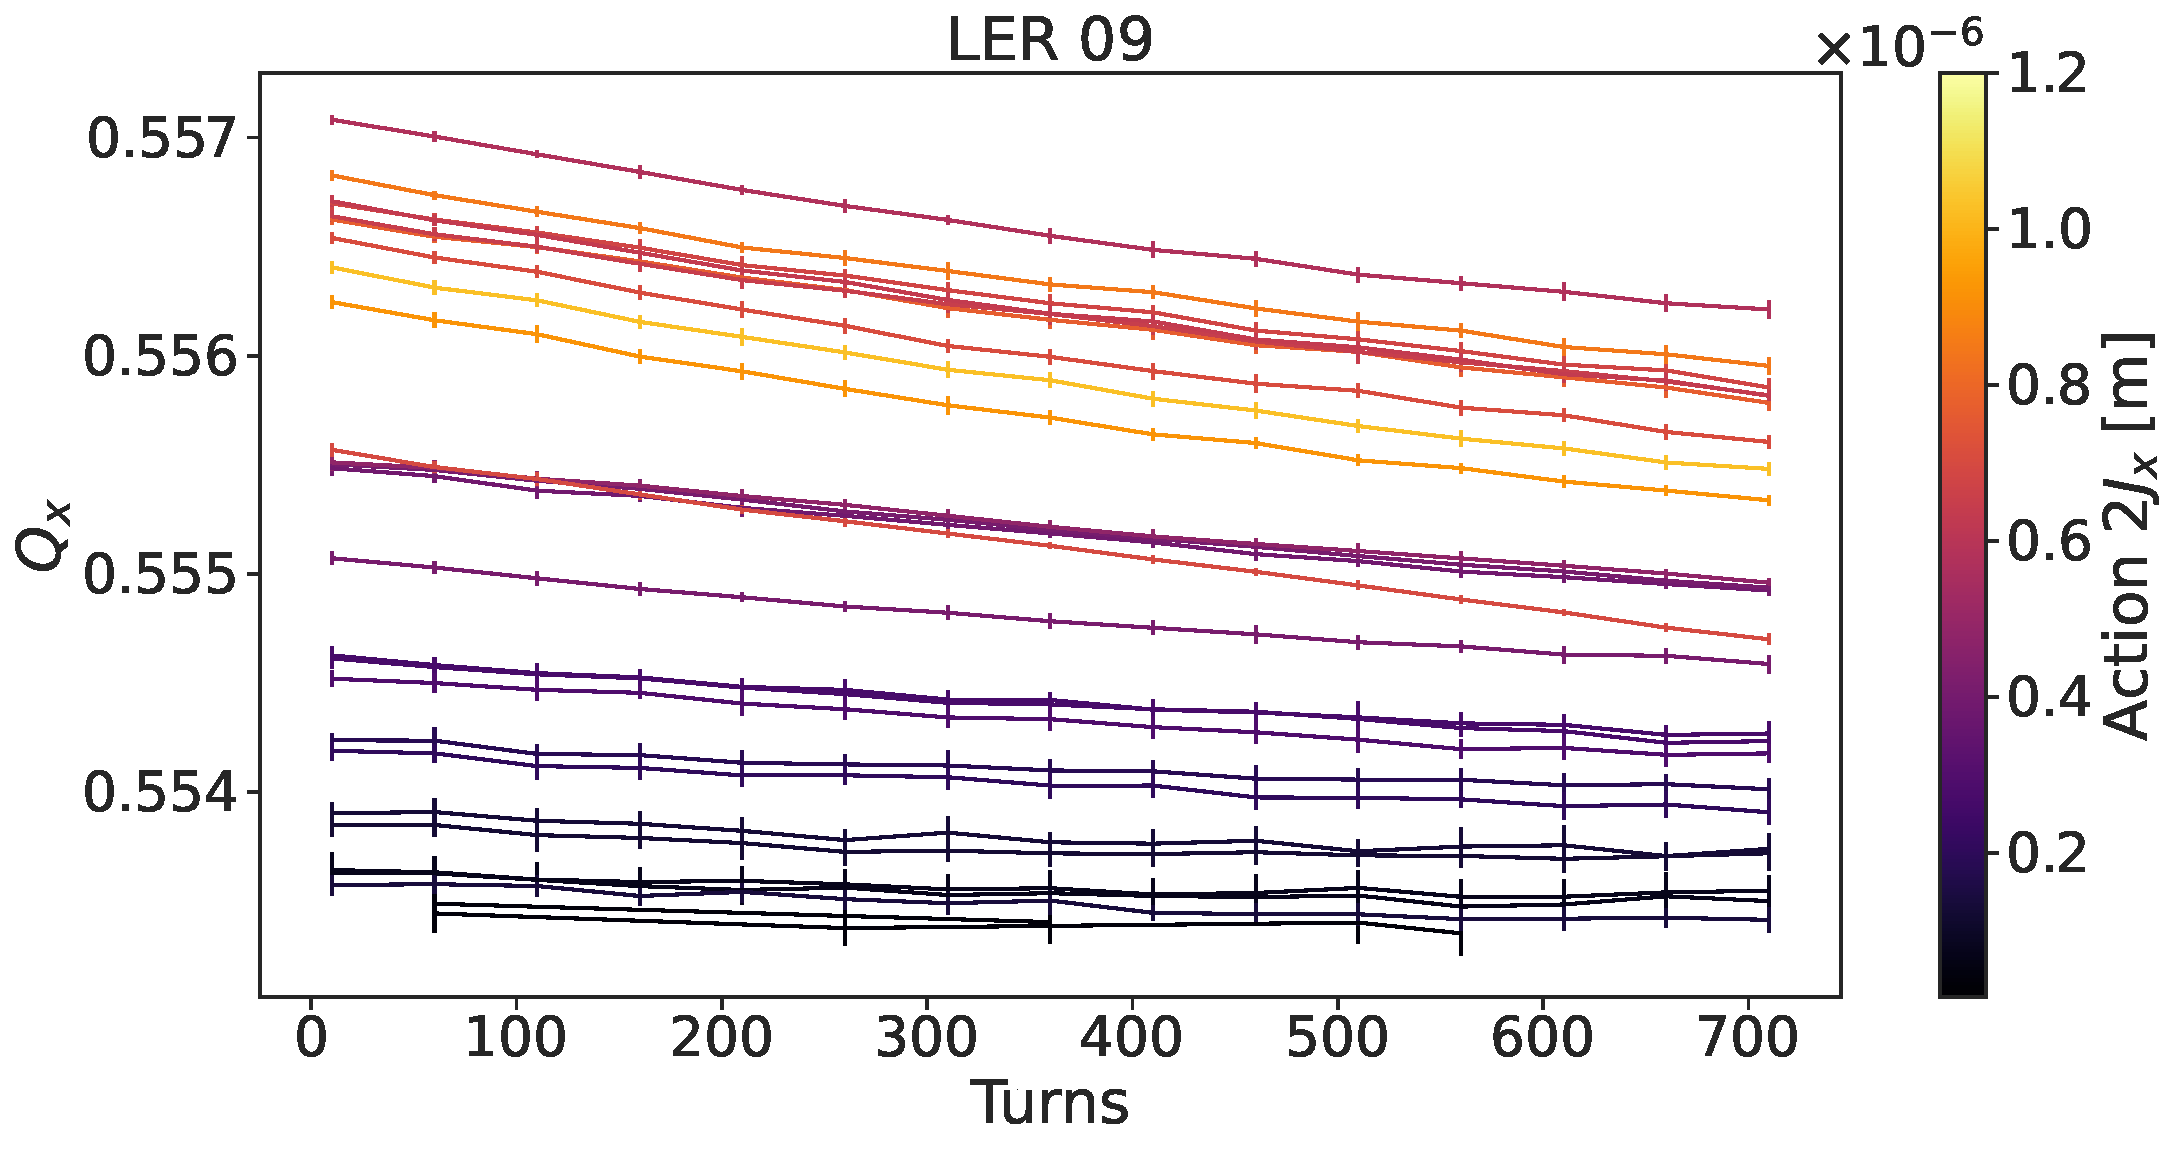
\includegraphics[width=0.8\linewidth]{images/kek/LER_detuned_ampdet.pdf}
    \caption{Correlation between the measured tune with the action of the kick. The tune is computed
    via a running window over 200 turns, every 50 turns.}
    \label{fig:kek:ler_full_tune_ampdet}
\end{figure}

The variation of the horizontal tune with the horizontal kick amplitude is related to by the
amplitude detuning term $\frac{\partial Q_x}{\partial J_x}$. Its value can be retrieved by fitting
the tune to the action. \Cref{fig:kek:ler_ampdet} shows the various kicks along with a fit and a
comparison to the model. The measured value, $6500 \pm 500$ is one order of magnitude higher than
that simulated, of $600$. This observed discrepancy indicates un-modeled octupolar-like sources.
Such a discrepancy, although not as large, already has been observed with different
optics~\cite{keintzel_jacqueline_beam_2022}.

\begin{figure}[!htb]
    \centering
    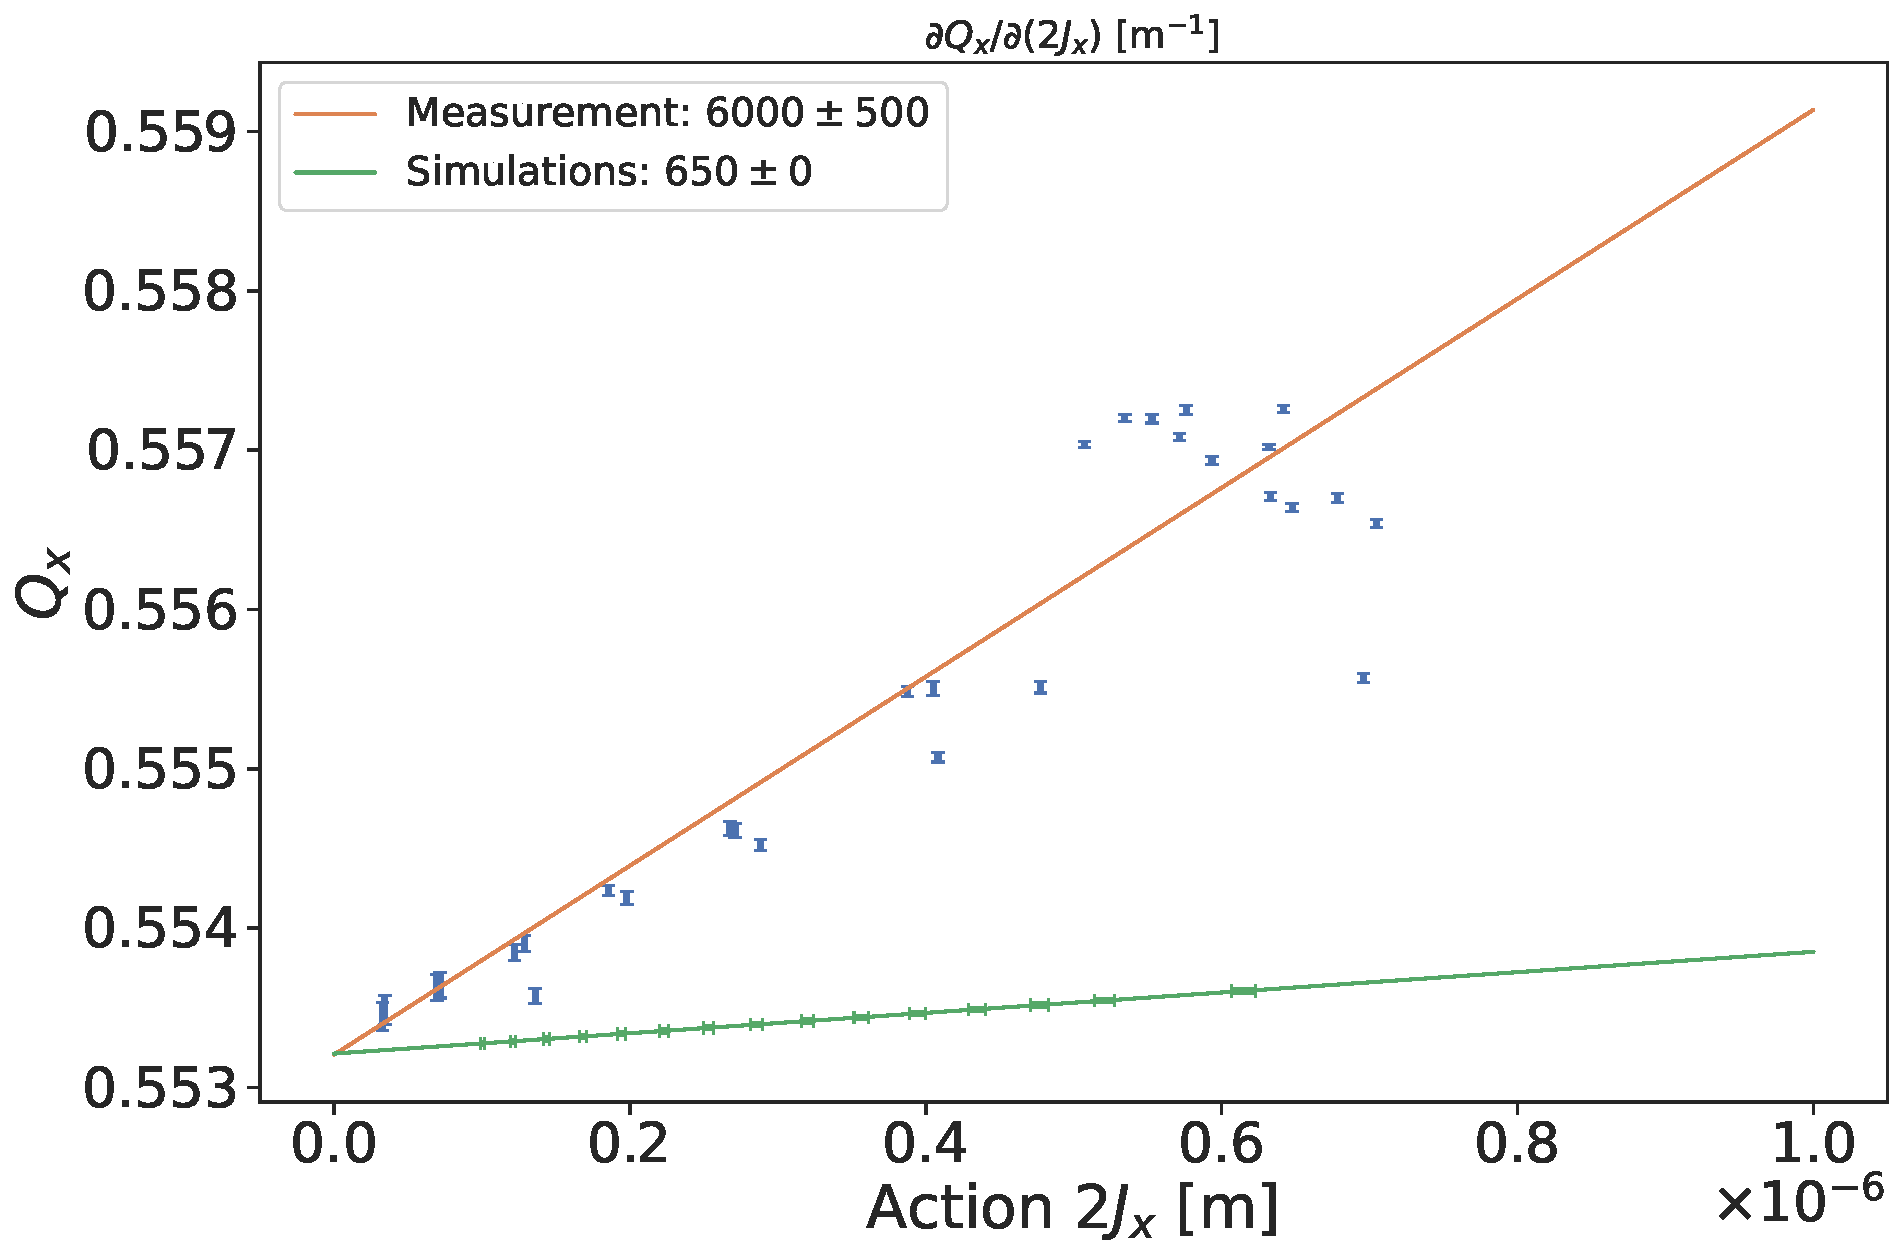
\includegraphics[width=0.7\linewidth]{images/kek/amplitude_detuning.pdf}
    \caption{Amplitude dependence of the tune in the LER ring. The fitted line then corresponds to
    the amplitude detuning term $\partial Q_x/\partial 2J_x$. For comparison, the model computed 
    from the model is shown in green.}
    \label{fig:kek:ler_ampdet}
\end{figure}



%-----------------------------
%   Resonance Driving Terms
%-----------------------------
\FloatBarrier
\subsection{\review{Resonance Driving Terms}}

Resonance Driving Terms, coefficients linked to the strength of a resonance, can be measured via
their associated line amplitude in the frequency spectrum. To reliably measure RDTs, these
line amplitudes must be clearly distinguishable and above the noise level for every BPM. This can be
challenging to achieve and often requires high amplitude kicks.
For example, lines in the vertical spectrum, attributed to octupoles, were previously
observed~\cite{keintzel_jacqueline_beam_2022} but could not lead to a succesful RDT measurement due
to kick amplitudes.

However, new measurements were taken with a different working point in order to be closer to the 
resonances with the hope of increasing their impact on particle motion. A resonance diagram,
illustrating those resonances and the typical working point of LER is shown in
\cref{fig:kek:tune_diagram}. Although several working points were tested, no clear correlation
between them and succesful RDTs measurements could be established. The main determining factor
remained the kick amplitude. A typical frequency spectrum from a succesful measurement in HER for
the vertical plane is shown in \cref{fig:kek:rdt_spectrum_HER}. The line $-1Q_x - 1Q_y$ is seen at
each BPM. Additionaly, lines near the vertical tune are attributed to the synchrotron tune.

\begin{figure}[!htb]
    \centering
    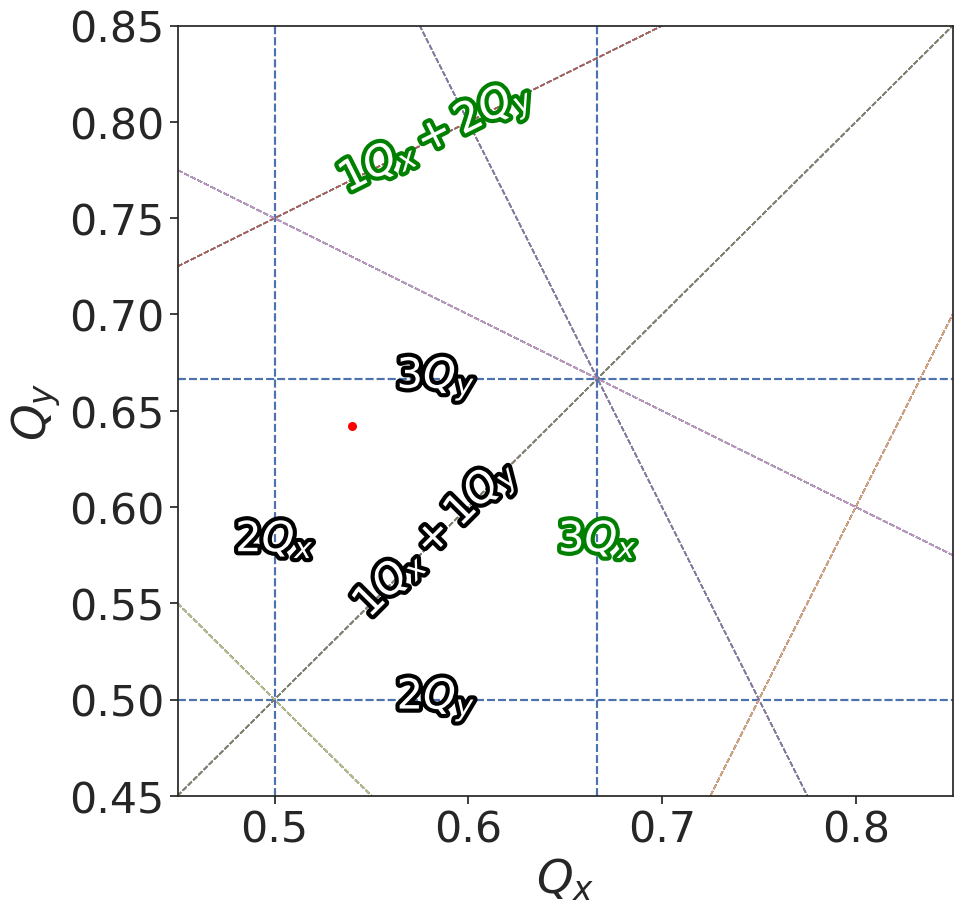
\includegraphics[width=0.6\linewidth]{images/kek/tune_diagram.png}
    \caption{Resonance diagram highlighting the resonances close to the HER working point, in red, 
    and those often visible in the frequency spectra, in green.}
    \label{fig:kek:tune_diagram}
\end{figure}

\begin{figure}[!htb]
    \centering
    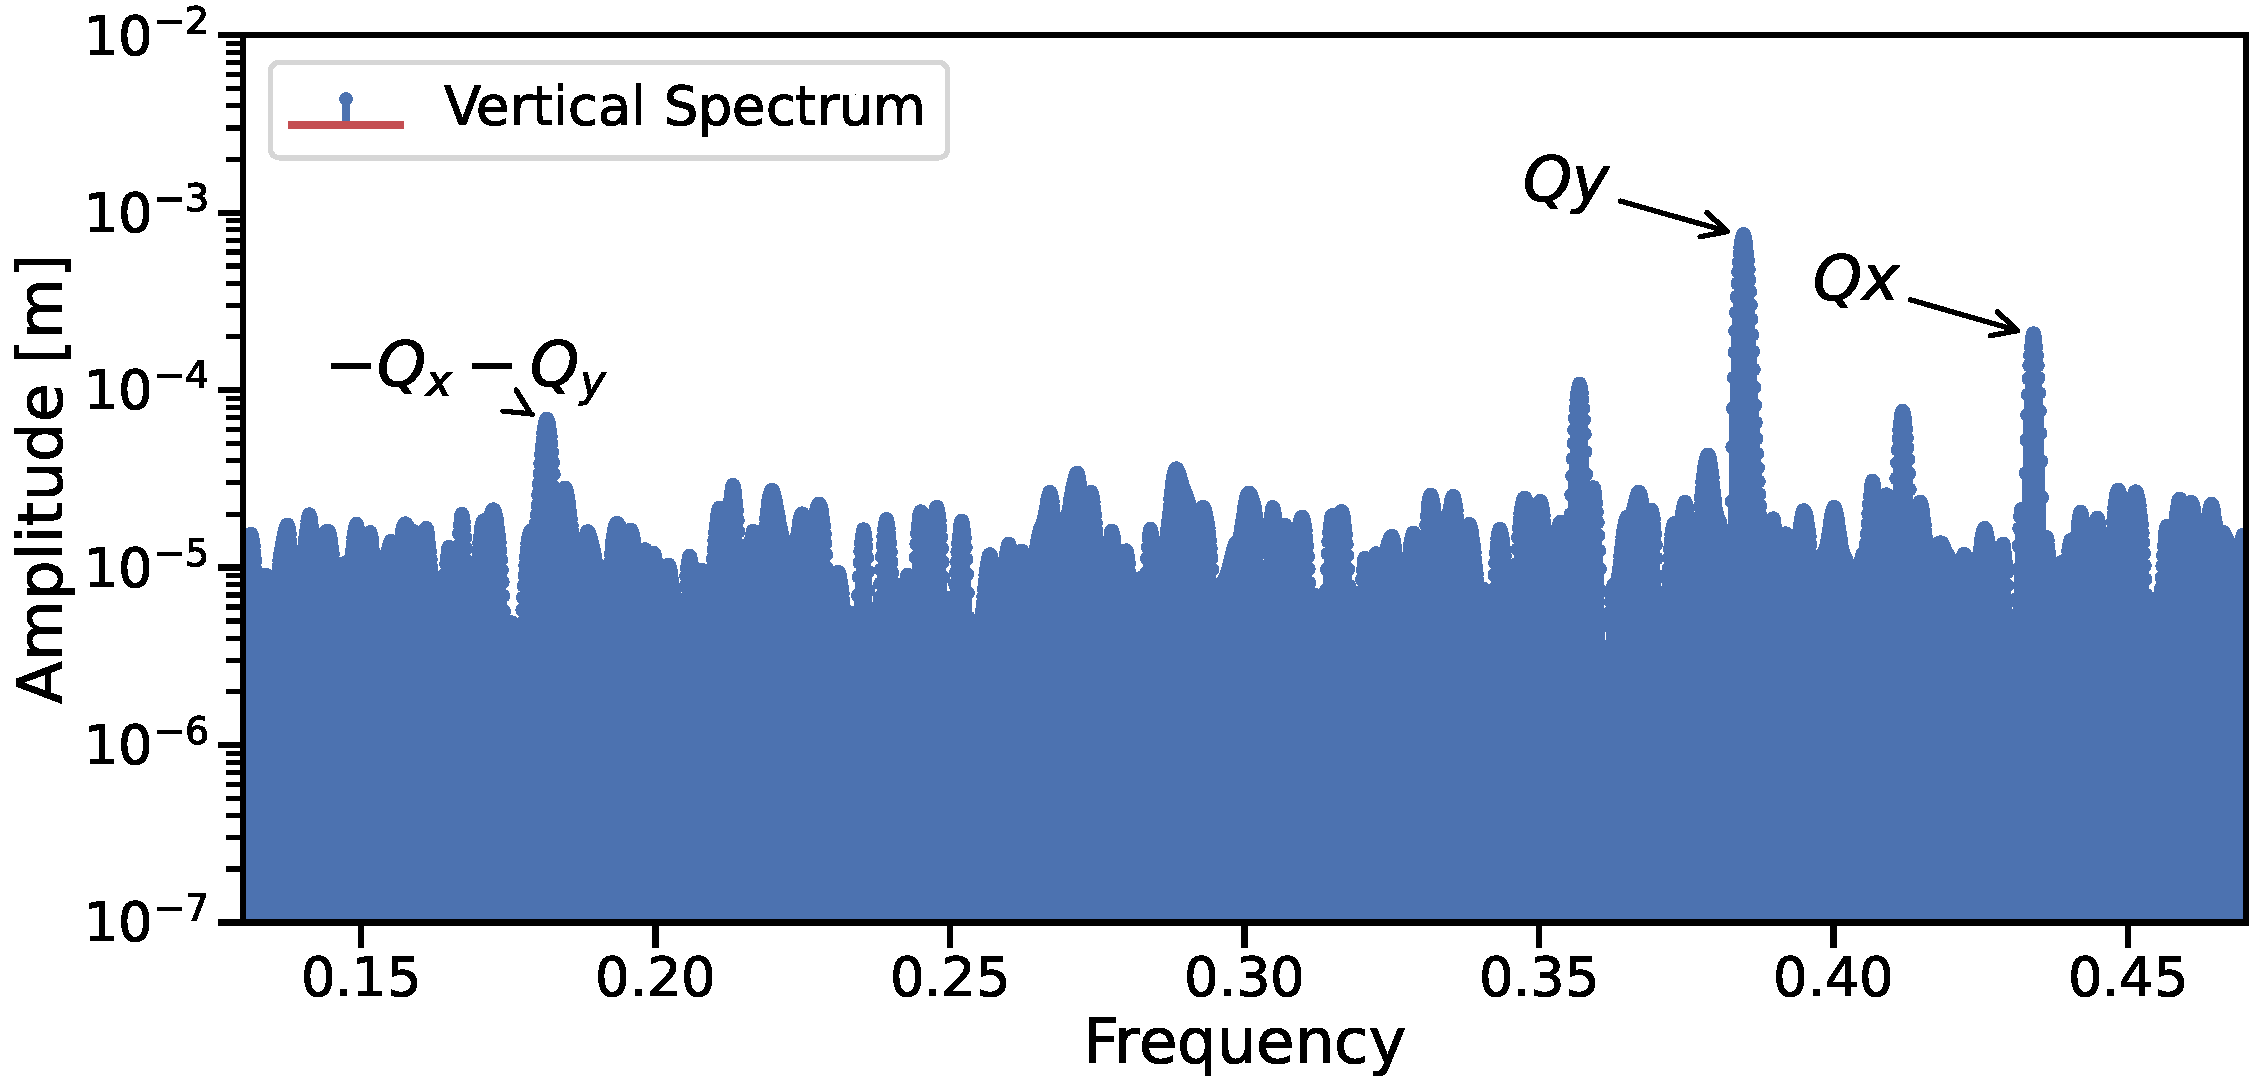
\includegraphics[width=0.8\linewidth]{images/kek/HER_2024-02-06_sextupoles_spectrum.pdf}
    \caption{}
    \label{fig:kek:rdt_spectrum_HER}
\end{figure}

Successful measurements of sextupolar RDTs were indeed obtained. Specifically,
the RDTs $f_{3000,x}$ in LER and $f_{1020,y}$ in HER were measured using the
\textit{detuned} optics configuration. While additional sextupolar lines were clearly visible in
both the horizontal and vertical spectra, no clear RDT measurements could be extracted. The measured
amplitudes, along with comparisons to the model, are presented in \cref{fig:kek:rdt_f3000x_LER} and
\cref{fig:kek:rdt_f1020y_HER}. Notably, both measurements exhibit discrepancies with the model. 
The average amplitude of $f_{1020}$ in the vertical plane for HER is measured at $21$, compared to a
modeled amplitude of $7$. Similarly, for $f_{3000}$, the average values measured in the horizontal
plane for LER are $2$ and $1.3$. These discrepancies remain largely unexplored and may arise from
decoherence effects that were not accounted for in the analysis software. additional, these could
also arise from contributions from other multipoles through feed-down or feed-up, as observed in the
LHC. The measured spikes in the HER RDT are not yet explained, but could come from a badly
reconstructed phase space due to non-optimal phase advances between BPMs in that region.

\begin{figure}[!htb]
    \centering
    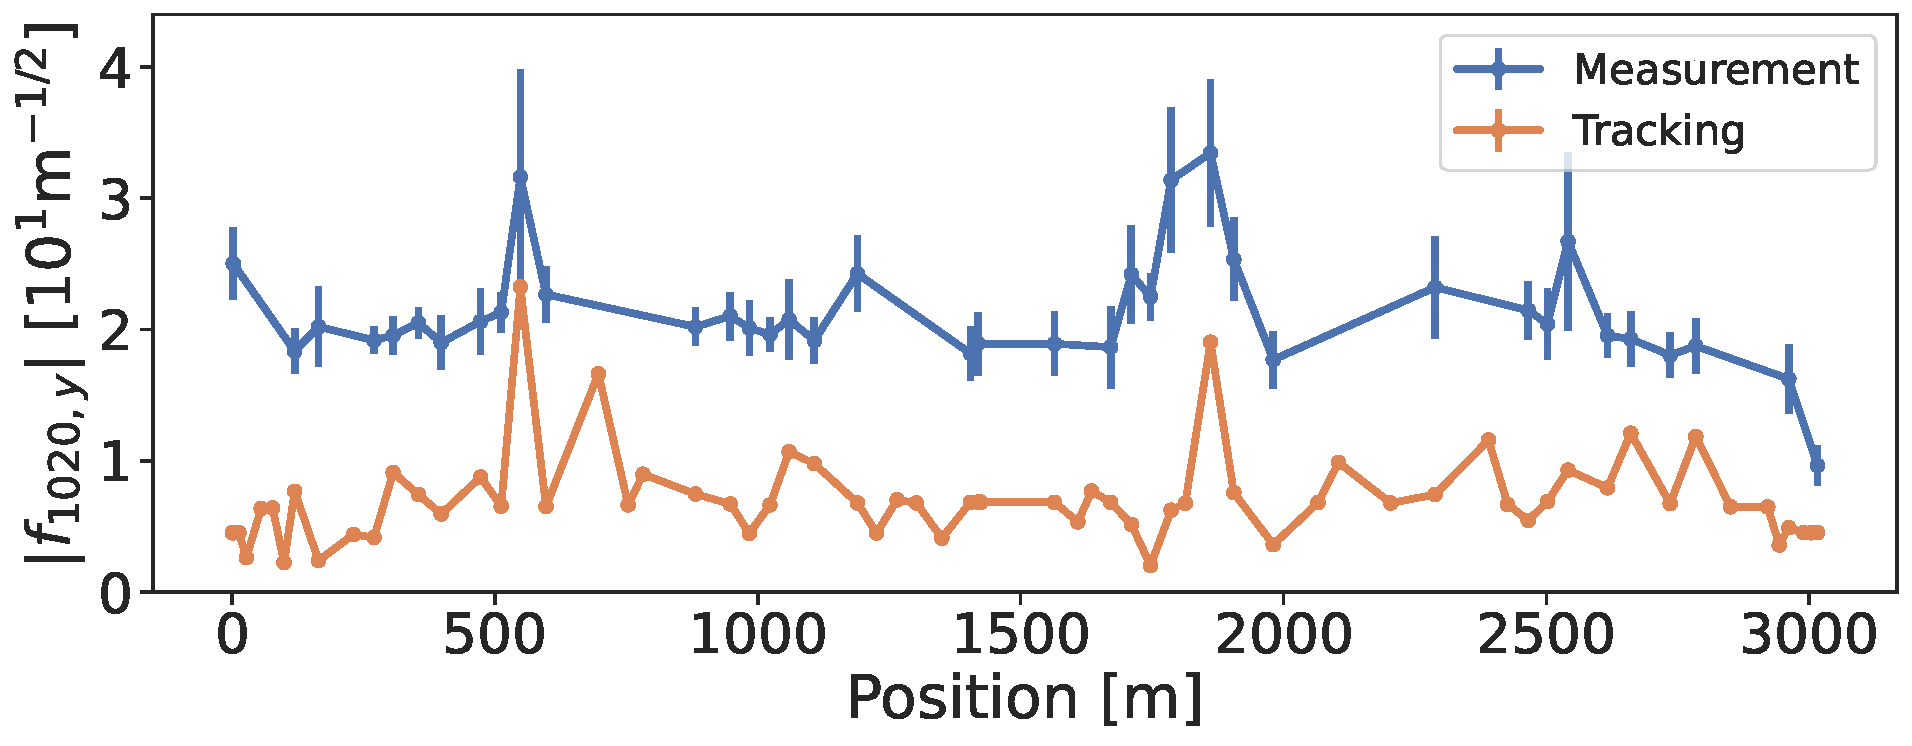
\includegraphics[width=0.8\linewidth]{images/kek/f1020y_HER.pdf}
    \caption{}
    \label{fig:kek:rdt_f1020y_HER}
\end{figure}

\begin{figure}[!htb]
    \centering
    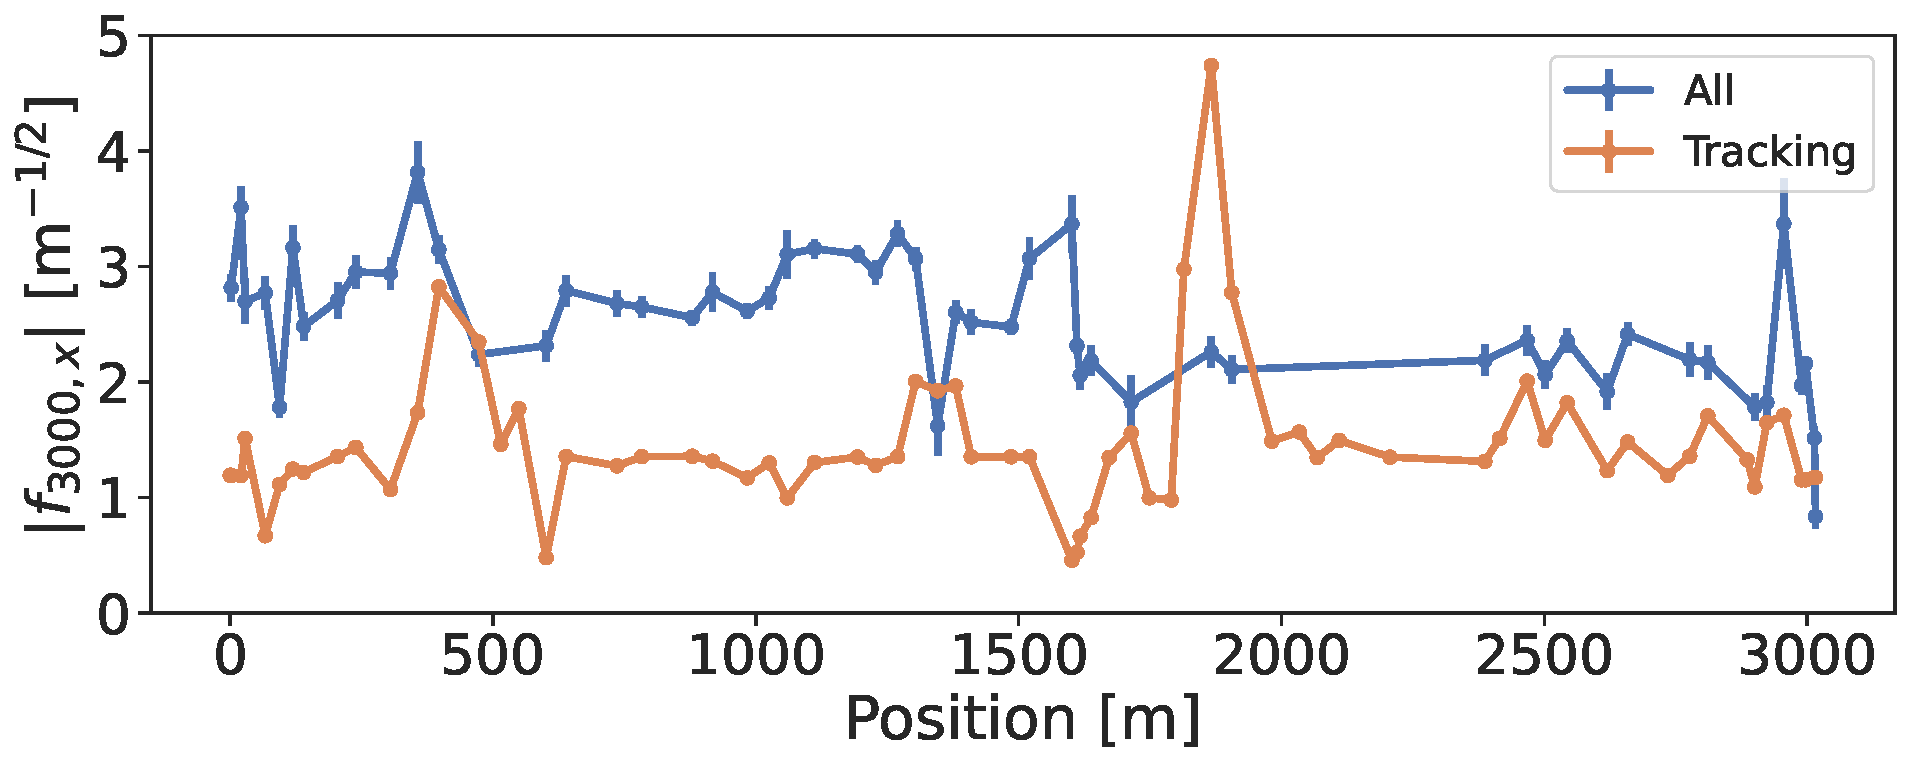
\includegraphics[width=0.8\linewidth]{images/kek/f3000x_LER.pdf}
    \caption{}
    \label{fig:kek:rdt_f3000x_LER}
\end{figure}



%-----------------------------
%        Chromaticity
%-----------------------------
\FloatBarrier
\subsection{\review{Chromaticity}}

Chromaticity measurements were performed using the method of varying the RF frequency, as described
in \cref{subsection:optics_corrections_chromaticity}. While this method is standard at the LHC, it
is not regularly used on the SuperKEKB rings. However, it provides the ability to measure the tune
over a broader range of momentum offsets. Chromaticity can also be computed using the Injection
Kicker~\cite{keintzel_jacqueline_beam_2022}. Similar to the LHC at injection energy, the Lorentz
factor $\gamma^{-2}$ is small compared to the momentum compaction factor $\alpha_c$ and can
therefore be neglected.
\Cref{fig:kek:chroma_procedure} illustrates the RF frequency method.

\begin{figure}[!htb]
    \centering
    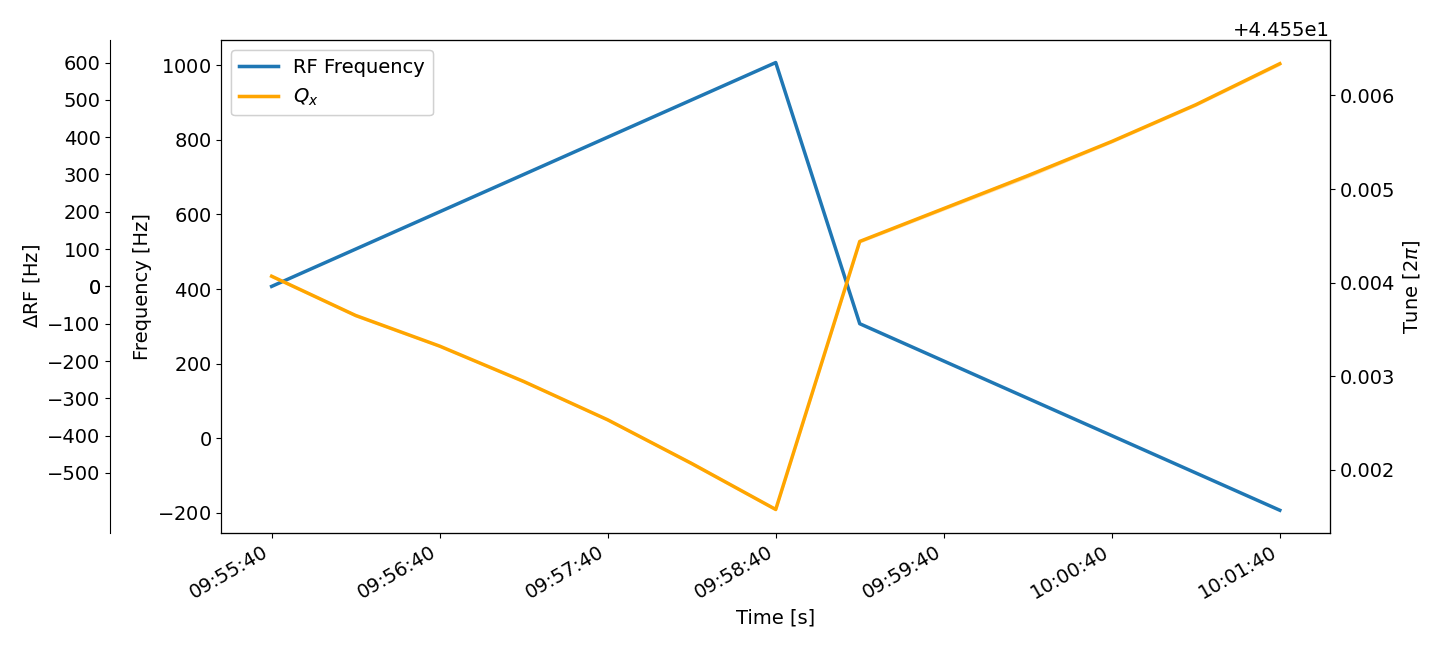
\includegraphics[width=0.8\linewidth]{images/kek/rf_qx.png}
    \caption{Horizontal tune change relative to the change in RF Frequency at SuperKEKB.}
    \label{fig:kek:chroma_procedure}
\end{figure}

Two measurements were taken with \textit{detuned} optics for the HER and LER rings and are shown 
in \cref{fig:kek:chroma_HER_detuned} and \cref{fig:kek:chroma_LER_detuned}. The values of the fitted
chromaticity function are given in \cref{tab:kek:her_chroma_detuned} and
\cref{tab:kek:ler_chroma_detuned} for HER and LER respectively. In order to allow for a better
comparison the tune and the linear chromaticity taken from the the measurements.

\begin{figure}[!htb]
    \centering
    \begin{subfigure}[b]{0.49\textwidth}
        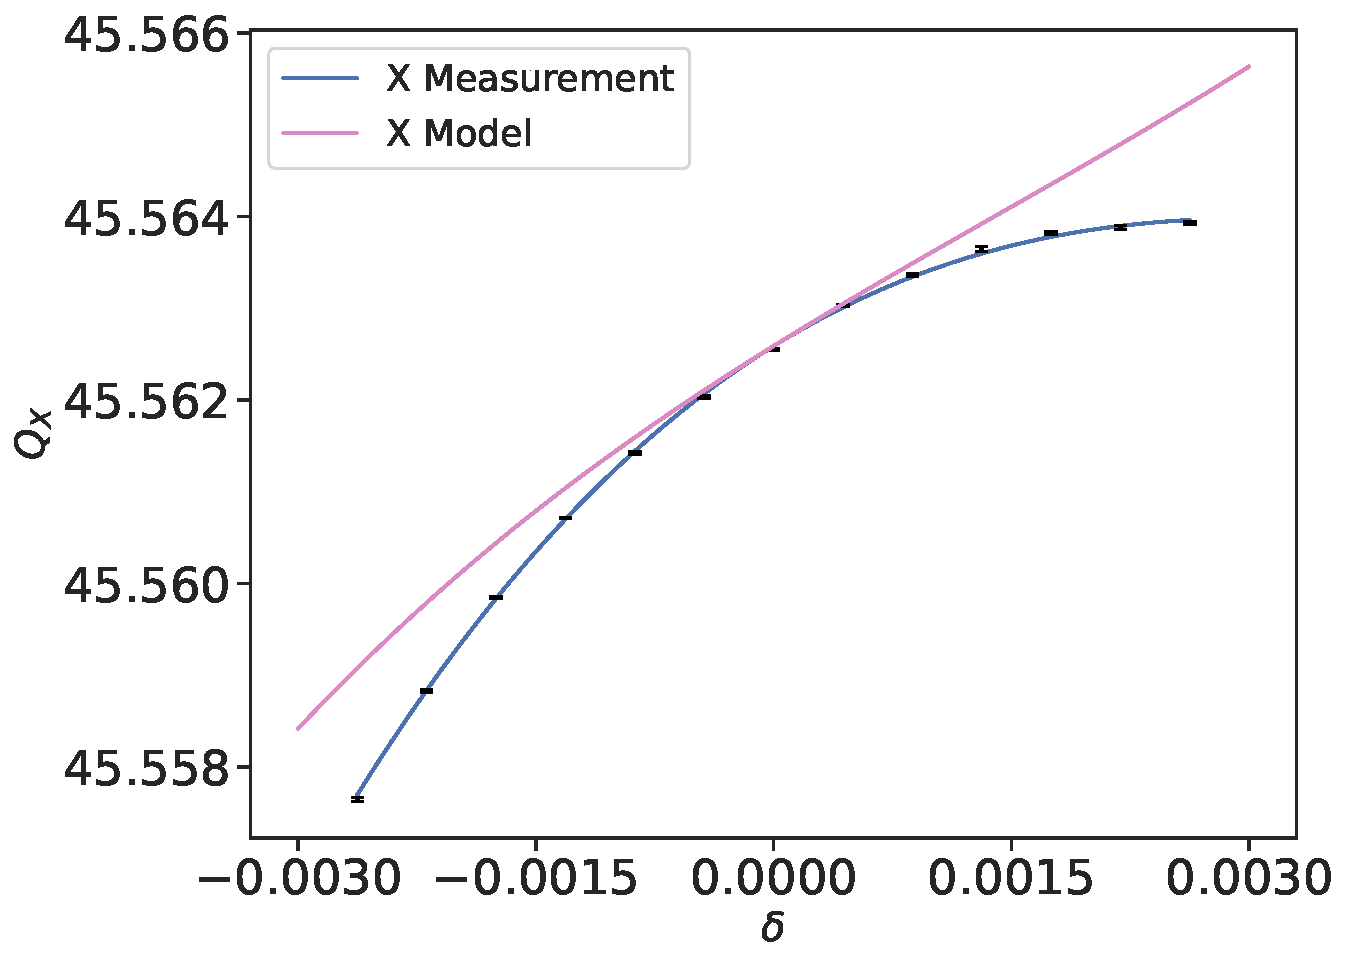
\includegraphics[width=\linewidth]{images/kek/chromaticity/HER_09/qx_modelq0q1.pdf}
        \caption{Horizontal tune shift.}
    \end{subfigure}
    \begin{subfigure}[b]{0.49\textwidth}
        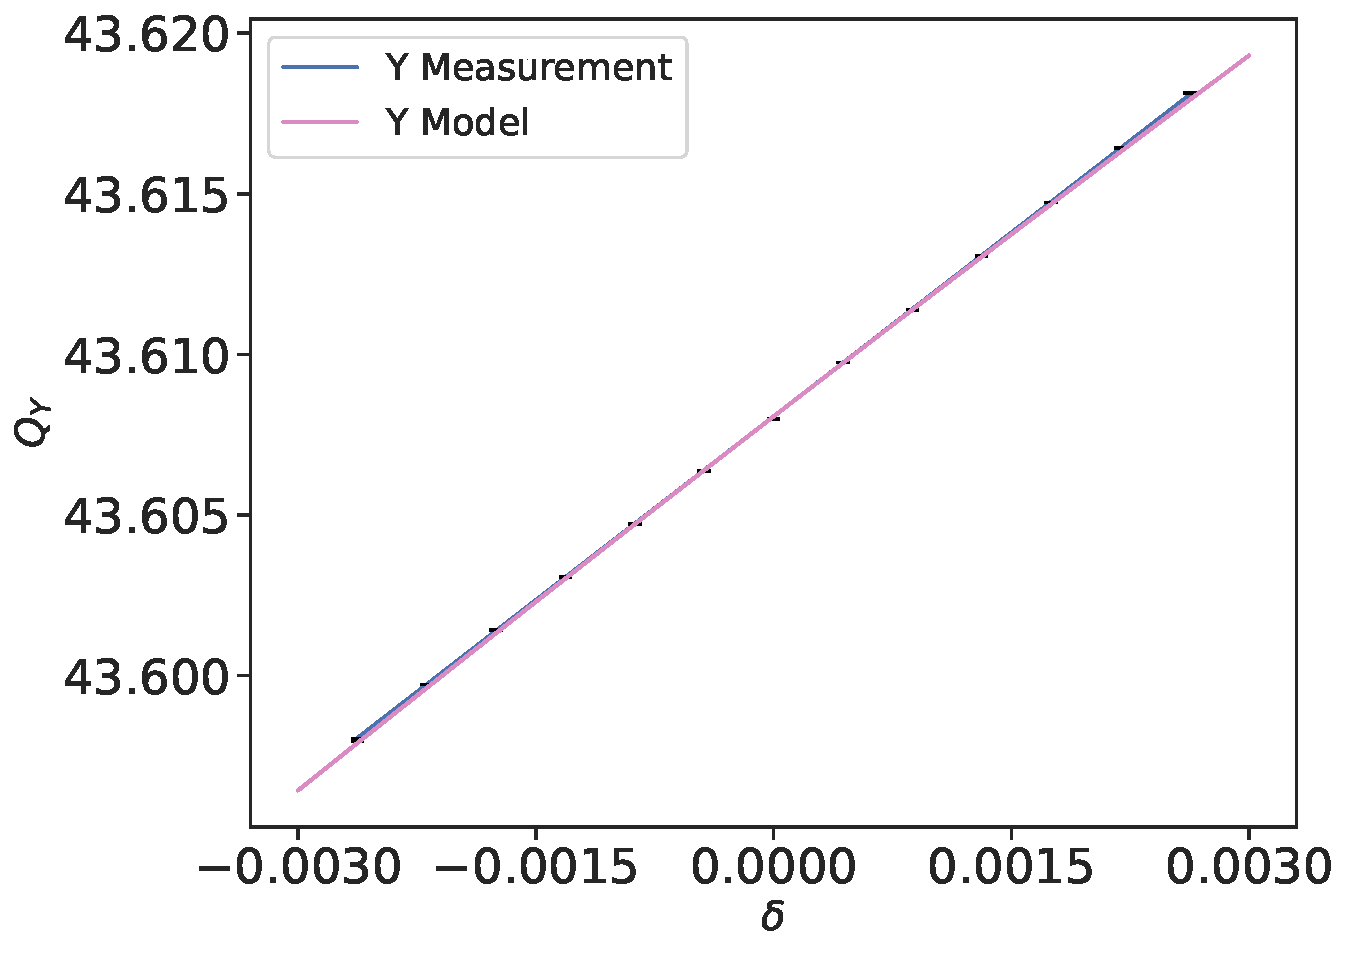
\includegraphics[width=\linewidth]{images/kek/chromaticity/HER_09/qy_modelq0q1.pdf}
        \caption{Vertical tune shift.}
    \end{subfigure}
    \caption{HER chromaticity measurements with \textit{detuned} optics.}
    \label{fig:kek:chroma_HER_detuned}
\end{figure}

\begin{figure}[!htb]
    \centering
    \begin{subfigure}[b]{0.49\textwidth}
        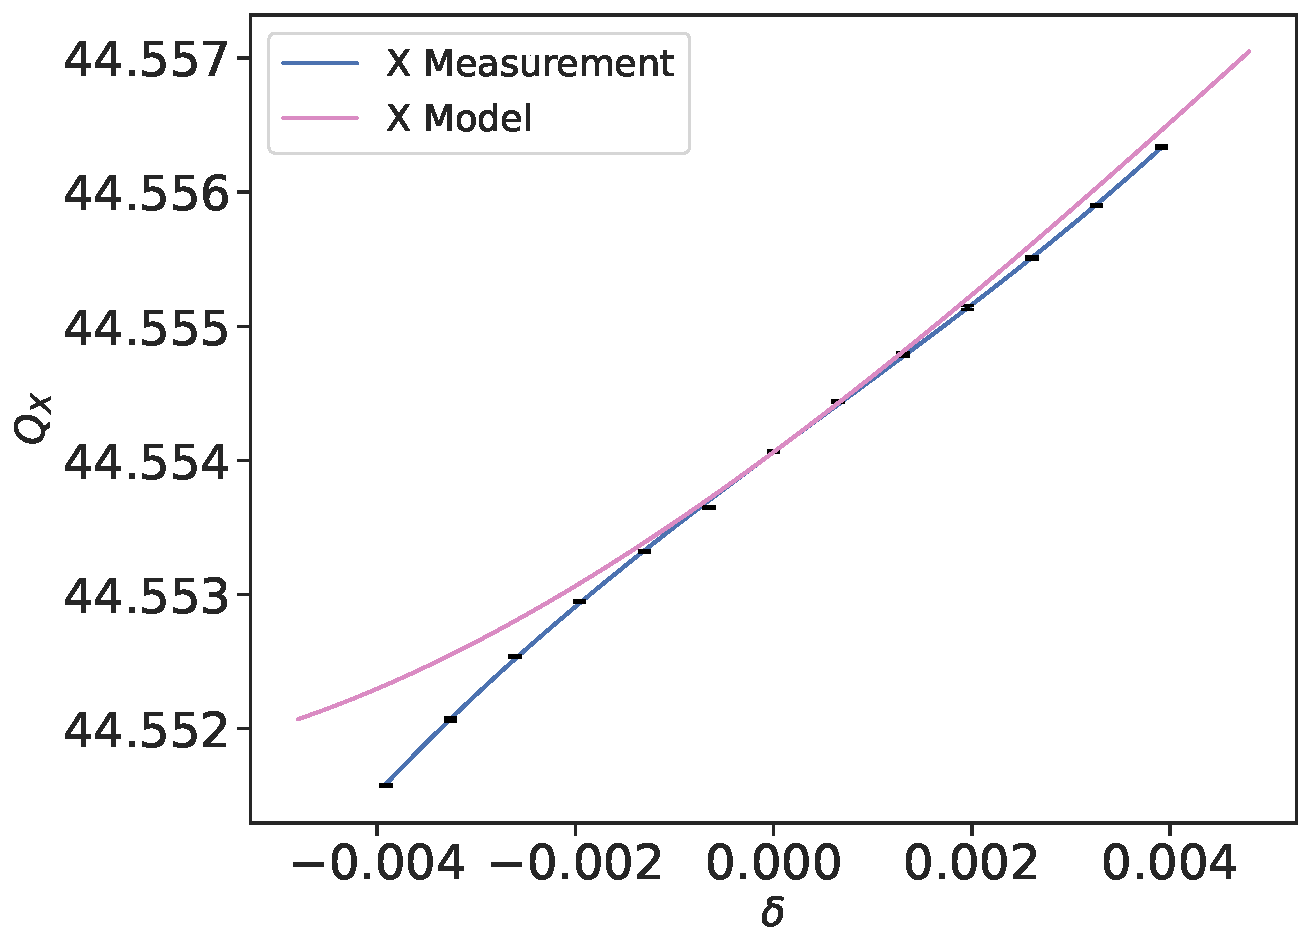
\includegraphics[width=\linewidth]{images/kek/chromaticity/LER_09/qx_modelq0q1.pdf}
        \caption{Horizontal tune shift.}
    \end{subfigure}
    \begin{subfigure}[b]{0.49\textwidth}
        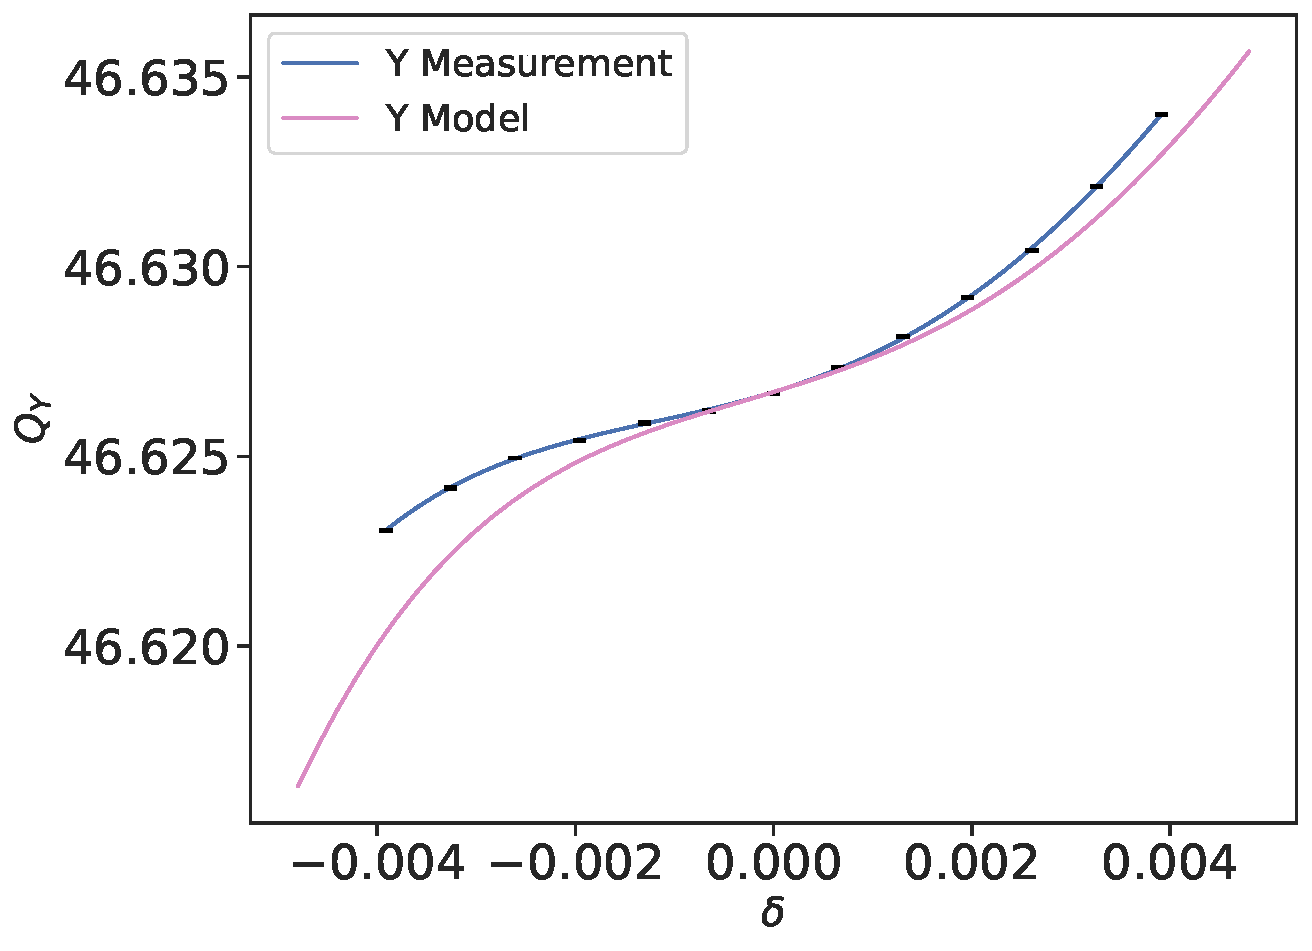
\includegraphics[width=\linewidth]{images/kek/chromaticity/LER_09/qy_modelq0q1.pdf}
        \caption{Vertical tune shift.}
    \end{subfigure}
    \caption{LER chromaticity measurements with \textit{detuned} optics.}
    \label{fig:kek:chroma_LER_detuned}
\end{figure}

% HER Detuned
\begin{table}[!htb]
    \centering
    \begin{tabular}{cccc}
        \toprule
            & & \(Q'' \, [\times 10^3]\) & \(Q''' \, [\times 10^6]\) \\ 
        \midrule
        \multirow{2}{*}{X} & Meas. & $-0.51 \pm 0.01$ & $0.11 \pm 0.02$ \\
                        & Model & $-0.12 \pm 0.00$ & $0.09 \pm 0.00$ \\
        \midrule
        \multirow{2}{*}{Y} & Meas. & $0.00 \pm 0.0$ & \\
                        & Model & $-0.04 \pm 0.0$ & \\
        \bottomrule
    \end{tabular}
    \caption{Measured and modeled chromaticity in the HER ring with \textit{detuned} optics in both
    planes.}
    \label{tab:kek:her_chroma_detuned}
\end{table}

% LER Detuned
\begin{table}[!htb]
    \centering
    \begin{tabular}{ccrrr}
        \toprule
            & & \(Q'' \, [\times 10^3]\) & \(Q''' \, [\times 10^6]\) & $Q^{(4)} [\times 10^9]$\\ 
        \midrule
        \multirow{2}{*}{X} & Meas. & $-0.01 \pm 0.0$ & $ 0.02 \pm 0.0$ \\
                        & Model & $ 0.04 \pm 0.0$ & $-0.01 \pm 0.0$ \\
        \midrule
        \multirow{2}{*}{Y} & Meas. & $0.35 \pm 0.01$ & $0.25 \pm 0.01$ & $-0.09 \pm 0.01$\\
                        & Model & $0.10 \pm 0.00$ & $0.32 \pm 0.00$ & $-0.09 \pm 0.00$ \\
        \bottomrule
    \end{tabular}
    \caption{Measured and modeled chromaticity in the LER ring with \textit{detuned} optics in both
    planes.}
    \label{tab:kek:ler_chroma_detuned}
\end{table}

It can be noted that most of the measured third and fourth-order chromaticities agree well with the
model, whereas the second-order chromaticity appears to deviate. Discrepancies in $Q''$ were
already observed in 2022 with different optics~\cite{keintzel_jacqueline_beam_2022}. This
discrepancy could arise from octupolar sources and higher-order contributions from sextupoles.



%=============================
 %        Conclusion
%=============================
\FloatBarrier
\section{\review{Summary}}

The measurements reveal excellent reproducibility of linear optics, with notable improvements in the
horizontal plane when a kicker is used. This consistency has been observed over multiple days and
across different shots. Sextupolar Resonance Driving Term (RDT) measurements have been carried out
in both rings for the first time, though some measurements were challenging to achieve, and certain
discrepancies remain unresolved. Chromaticity measurements for both rings were generally
satisfactory, but some inconsistencies in $Q''$ were observed in both the HER and LER.

Amplitude detuning for the LER was measured with detuned optics, and the model comparison showed an
order of magnitude difference. Combined with the chromaticity results, this suggests potential
errors due to higher-order effects of sextupoles and octupoles. Further investigations are needed to
clarify these discrepancies.

Overall, the measurements are consistent with those obtained using different methods at KEK. This
suggests that the techniques employed at CERN are effective and could enhance our understanding of
the machine and its modeling.